% ***********************************************************
% Dissertation template and document class for
%           The Hong Kong Polytechnic University
% Author  : QING Pei <edwardtoday@gmail.com>
% Adapted from: http://engineering.purdue.edu/~mark/puthesis/
% ***********************************************************


%%% For the electronic copy, use doublespacing,
%   define "\printmode" to get all text black for readability
\documentclass[12pt,lot,lof]{hkputhesis}
\newcommand{\printmode}{}

%%% For early drafts without some of the frontmatter
% Also see the "ifodd" command below to disable more frontmatter
%\documentclass[12pt]{hkputhesis}

%%% The PDF version should be compatible with Acrobat 5.0 or above
%   which make it PDF 1.4
% \pdfoutput=1
\pdfminorversion=4
\pdfobjcompresslevel=0
% \pdfimageresolution=300
% \pdfpkresolution=300
% or you could simply use a package to achieve this
% \RequirePackage{pdf14}

%%%%%%%%%%%%%%%%%%%%%%%%%%%%%%%%%%%%%%%%%%%%%%%%%%%%%%%%%%%%%
%%%% Author & title page info

\title{Palmprint Recognition with Three Dimensional Features}

\submitted{June 2012}  % degree conferral date (January, April, June, September, or November)
\copyrightyear{2012}  % year in which the copyright is secured by publication of the dissertation.
\author{QING Pei}
% \adviser{David Zhang}  %replace with the full name of your adviser
% \departmentprefix{Program in}  % defaults to "Department of", but programs need to change this.
% \department{Computing}
\programme{Master of Science in Software Technology}

%%%%%%%%%%%%%%%%%%%%%%%%%%%%%%%%%%%%%%%%%%%%%%%%%%%%%%%%%%%%%
%%%% Tweak float placements
% From: http://mintaka.sdsu.edu/GF/bibliog/latex/floats.html "Controlling LaTeX Floats"
% and based on: http://www.tex.ac.uk/cgi-bin/texfaq2html?label=floats
% LaTeX defaults listed at: http://people.cs.uu.nl/piet/floats/node1.html

% Alter some LaTeX defaults for better treatment of figures:
  % See p.105 of "TeX Unbound" for suggested values.
  % See pp. 199-200 of Lamport's "LaTeX" book for details.
  %   General parameters, for ALL pages:
  \renewcommand{\topfraction}{0.85}	% max fraction of floats at top
  \renewcommand{\bottomfraction}{0.6}	% max fraction of floats at bottom
  %   Parameters for TEXT pages (not float pages):
  \setcounter{topnumber}{2}
  \setcounter{bottomnumber}{2}
  \setcounter{totalnumber}{4}     % 2 may work better
  \setcounter{dbltopnumber}{2}    % for 2-column pages
  \renewcommand{\dbltopfraction}{0.66}	% fit big float above 2-col. text
  \renewcommand{\textfraction}{0.15}	% allow minimal text w. figs
  %   Parameters for FLOAT pages (not text pages):
  \renewcommand{\floatpagefraction}{0.66}	% require fuller float pages
	% N.B.: floatpagefraction MUST be less than topfraction !!
  \renewcommand{\dblfloatpagefraction}{0.66}	% require fuller float pages

% The documentclass already sets parameters to make a high penalty for widows and orphans.

%%%%%%%%%%%%%%%%%%%%%%%%%%%%%%%%%%%%%%%%%%%%%%%%%%%%%%%%%%%%%
%%% Use packages

\usepackage{amsfonts,amsmath}

%%% For figures
\usepackage{graphicx,epstopdf,subfigure}

%%% for comments and listings
\usepackage{verbatim}

%%% For tables
\usepackage{multirow}

% Longtable lets you have tables that span multiple pages.
\usepackage{longtable}
\usepackage{lscape}
\usepackage[tableposition=top]{caption}
\captionsetup[table]{labelsep=period}  % Change colon in "Table ##:" to "."

% Booktabs produces far nicer tables than the standard LaTeX tables.
%   see: http://en.wikibooks.org/wiki/LaTeX/Tables
\usepackage{booktabs}

%set parameters for longtable:
% default caption width is 4in for longtable, but wider for normal tables
\setlength{\LTcapwidth}{\textwidth}

%%% Date formatting
\usepackage{datetime}

%%% Set fonts
% defines Adobe Times Roman (or equivalent) as default text font
\usepackage{mathptmx}

%%% Set line spacing
\usepackage{setspace}
\onehalfspacing

%%% Turn off indentation globally
\usepackage{parskip}
\setlength{\parskip}{18pt} % to simulate a blank line between paragraphs

%%% Page number at bottom right
\usepackage{fancyhdr}
\fancyhf{} % clear all header and footers
\renewcommand{\headrulewidth}{0pt} % remove the header rule
\rfoot{\fancyplain{\minsize\thepage\hspace{1.8em}}{\minsize\thepage\hspace{1.8em}}}
\pagestyle{fancyplain}

%%% Create hyperlinks for cross-references in the document.
\usepackage{hyperref}
\hypersetup{bookmarksnumbered}
% copy the already-set title and author to use in the pdf properties
\makeatletter
\hypersetup{pdftitle=\@title,pdfauthor=\@author,pdfcreator=\@author}
\makeatother

%%% Setting the margins
\usepackage[top=1in, left=1.8in, bottom=1.4in, right=1.1in]{geometry}

%%% Change chapter heading format (with text shadow)
\usepackage{shadowtext}
\shadowoffsetx{1pt}
\shadowoffsety{.7pt}
\usepackage{titlesec}
\makeatletter
\renewcommand{\@makechapterhead}[1]{%
\vspace*{-6pt}{\setlength{\parindent}{0pt} \raggedright \normalfont
\bfseries\chaptersize \shadowtext{\chaptertitlename\ \thechapter \quad\ #1
}}\vspace*{22pt}}
\makeatother

% change fontsize for section/subsection/subsubsection headings
\titleformat{\section}{\normalfont\sectionsize}{\thesection}{1em}{}
\titleformat{\subsection}{\normalfont\subsectionsize}{\thesubsection}{1em}{}
\titleformat{\subsubsection}{\normalfont\subsubsectionsize}{\thesubsection}{1em}{}

% Change spacing for headings. Please ignore the actual numbers.
% They are tweaked by comparing PDF outputs to the Word template. --!
\titlespacing*{\section}{0pt}{-12pt}{6pt}
\titlespacing*{\subsection}{0pt}{-14pt}{6pt}
\titlespacing*{\subsubsection}{0pt}{-16pt}{6pt}

%%% Change heading format of References
\renewcommand*{\bibname}{References}
\makeatletter
\renewenvironment{thebibliography}[1]{
\clearpage
\ifdefined\phantomsection
\phantomsection
\else
\fi
\addcontentsline{toc}{chapter}{\bibname}
\vspace*{-12pt}
\begin{doublespace}
  {\subsectionsize\bfseries \bibname}
\end{doublespace}
\vspace*{6pt}
\onehalfspacing
\@mkboth{\MakeUppercase\bibname}{\MakeUppercase\bibname}%
\list{\@biblabel{\@arabic\c@enumiv}}{
  \settowidth\labelwidth{\@biblabel{#1}}%
  \leftmargin\labelwidth
  \advance\leftmargin\labelsep
  \@openbib@code
  \usecounter{enumiv}%
  \let\p@enumiv\@empty
  \renewcommand\theenumiv{\@arabic\c@enumiv}}%
\sloppy
\clubpenalty4000
\@clubpenalty \clubpenalty
\widowpenalty4000%
\sfcode`\.\@m}{
  \def\@noitemerr
  {\@latex@warning{Empty `thebibliography' environment}}%
  \endlist}
 \makeatother

%%% Set heading format for Appendix
\usepackage{appendix}
\usepackage{appendix}
\makeatletter
\newcommand\appendix@chapter[1]{
	\refstepcounter{chapter}
	\orig@chapter*{
		\vspace*{-72pt}
		\subsectionsize\bfseries Appendix \@Alph\c@chapter: #1
		\vspace*{-36pt}
	}
	\addcontentsline{toc}{chapter}{Appendix \@Alph\c@chapter: #1}
}
\let\orig@chapter\chapter
\g@addto@macro\appendix{\let\chapter\appendix@chapter}
\makeatother


%%% Set Table of Contents format
\renewcommand\contentsname{Table of Contents}
\usepackage[subfigure]{tocloft}
\renewcommand{\cftbeforechapskip}{0pt}
\renewcommand{\cftbeforetoctitleskip}{6pt}
\renewcommand{\cftaftertoctitleskip}{12pt}
% Set ToC heading size the same as that of Abstract
\renewcommand\cfttoctitlefont{\subsectionsize\bfseries}
\renewcommand\cftchapfont{\tocchapsize\bfseries}
\renewcommand\cftchappresnum{Chapter } % prefix "Chapter " to chapter number in ToC
\cftsetindents{chapter}{0em}{5em}      % set amount of indenting
\makeatletter \renewcommand{\@dotsep}{1} \makeatother
\renewcommand{\cftchapdotsep}{\cftdotsep}

\renewcommand{\cftbeforeloftitleskip}{6pt}
\renewcommand{\cftafterloftitleskip}{18pt}
\renewcommand\cftloftitlefont{\subsectionsize\bfseries}
\renewcommand\cftfigpresnum{Figure }  % prefix "Figure " to entries in LoF
\cftsetindents{figure}{0em}{5em}      % set amount of indenting

\renewcommand{\cftbeforelottitleskip}{6pt}
\renewcommand{\cftafterlottitleskip}{18pt}
\renewcommand\cftlottitlefont{\subsectionsize\bfseries}
\renewcommand\cfttabpresnum{Table }	 % prefix "Table " to entries in LoT
\cftsetindents{table}{0em}{5em}      % set amount of indenting


%%%%%%%%%%%%%%%%%%%%%%%%%%%%%%%%%%%%%%%%%%%%%%%%%%%%%%%%%%%%%
%%% Printed vs. online formatting

\ifdefined\printmode
% url package understands urls (with proper line-breaks) without hyperlinking them
\usepackage{url}
% turn off code highlighting
\usepackage{listings}
\lstset{language=Matlab,
   keywords={break,case,catch,continue,else,elseif,end,for,function,
      global,if,otherwise,persistent,return,switch,try,while},
   basicstyle=\ttfamily,
   keywordstyle=\bfseries\color{black},
   commentstyle=\color{black},
   stringstyle=\color{black},
   numbers=left,
   numberstyle=\tiny\color{black},
   stepnumber=1,
   numbersep=10pt,
   backgroundcolor=\color{white},
   tabsize=4,
   showspaces=false,
   showstringspaces=false}
\else
% Online copy
% turn on code highlighting
\usepackage{color}
\usepackage{listings}
\definecolor{dkgreen}{rgb}{0,0.6,0}
\definecolor{gray}{rgb}{0.5,0.5,0.5}
\lstset{language=Matlab,
   keywords={break,case,catch,continue,else,elseif,end,for,function,
      global,if,otherwise,persistent,return,switch,try,while},
   basicstyle=\ttfamily,
   keywordstyle=\color{blue},
   commentstyle=\color{gray},
   stringstyle=\color{dkgreen},
   numbers=left,
   numberstyle=\tiny\color{red},
   stepnumber=1,
   numbersep=10pt,
   backgroundcolor=\color{white},
   tabsize=4,
   showspaces=false,
   showstringspaces=false}

% make the page number rather than the text be the link for ToC entries
%\hypersetup{linktocpage}

\fi % print or online formatting


%%%%%%%%%%%%%%%%%%%%%%%%%%%%%%%%%%%%%%%%%%%%%%%%%%%%%%%%%%%%%
%%%% Define commands

% Define any custom commands that you want to use.
% For example, highlight notes for future edits to the thesis
%\newcommand{\todo}[1]{\textbf{\emph{TODO:}#1}}


% create an environment that will indent text
% see: http://latex.computersci.org/Reference/ListEnvironments
% 	\raggedright makes them left aligned instead of justified
\newenvironment{indenttext}{
\begin{list}{}{ \itemsep 0in \itemindent 0in
\labelsep 0in \labelwidth 0in
\listparindent 0in
\topsep 0in \partopsep 0in \parskip 0in \parsep 0in
\leftmargin 1em \rightmargin 0in
\raggedright
}
\item
}
{\end{list}}

% another environment that's an indented list, with no spaces
% between items -- if we want multiple items/lines. Useful in
% tables. Use \item inside the environment.
% \raggedright makes them left aligned instead of justified
\newenvironment{indentlist}{
\begin{list}{}{ \itemsep 0in \itemindent 0in
\labelsep 0in \labelwidth 0in
\listparindent 0in
\topsep 0in \partopsep 0in \parskip 0in \parsep 0in
\leftmargin 1em \rightmargin 0in
\raggedright
}

}
{\end{list}}



%%%%%%%%%%%%%%%%%%%%%%%%%%%%%%%%%%%%%%%%%%%%%%%%%%%%%%%%%%%%%
%%%% Front-matter

% For early drafts, you may want to disable some of the frontmatter.
% Simply change this to "\ifodd 1" to do so.
\ifodd 0
% front-matter disabled while writing chapters
\renewcommand{\maketitlepage}{}
\renewcommand*{\makeauthorshipstatement}{}
\renewcommand*{\makeabstract}{}

% you can just skip the \acknowledgements and \dedication commands
% to leave out these sections.

\else

\abstract{
% Import the abstract file.
%!TEX root = thesis.tex

Three Dimensional (3D) palmprint has proved to be a significant biometrics for personal authentication. 3D palmprints are harder to counterfeit than 2D palmprints and more robust to variations in illumination and serious scrabbling on the palm surface. Previous work on 3D palmprint recognition has concentrated on local features such as texture and lines.

% a blank line as required
\vspace{12pt}

In this dissertation, the authentication process are improved using 3D features. The features are stable in samples from a single person over time and distinguishable among samples from different people. Three features adopted are Maximum Depth of palm center, Horizontal Cross-section Area and Radial Line Length from the centroid to the boundary of 3D palmprint horizontal cross-section of different levels. The feature set is combined as a column feature vector for matching. Support Vector Machine is introduced for higher efficiency.

% a blank line as required
\vspace{12pt}

Experiments are conducted on an existing 3D palmprint database of 8,000 samples. The results show that the proposed method is able to achieve an reasonable performance.


% \textbf{Keywords}: 3D palmprint identification, 3D palmprint verification, SVM

}

\acknowledgements{
%I would like to thank...
I would like to thank the Math department for providing the original documentclass file that this class is based upon. I would like to thank my parents, without whom my life would not be possible. I would also like to thank my advisor, my dissertation committee, and my research collaborators because every graduate student needs to do so. And finally, I thank the members of my research group, to whom I leave this template to save you some of the trouble I had to go through getting my dissertation to compile in \LaTeX{}.  

Don't forget to ask your advisor if your work was sponsored by a grant that needs to be acknowledged in this section.  
}

\dedication{To my parents.}

\fi  % disable frontmatter


%%%%%%%%%%%%%%%%%%%%%%%%%%%%%%%%%%%%%%%%%%%%%%%%%%%%%%%%%%%%%
%%%% Hide some chapters

%%% If you want to produce a pdf that includes only certain chapters, specify
%   them with includeonly, in addition to including all chapters below.
%\includeonly{ch-intro/chapter-intro}
%%% You can also specify multiple chapters.
%\includeonly{ch-intro/chapter-intro,ch-usage/chapter-usage}
%\includeonly{chap1,chap2,chap3}


%%%%%%%%%%%%%%%%%%%%%%%%%%%%%%%%%%%%%%%%%%%%%%%%%%%%%%%%%%%%%
%%%% Notes:

% Footnotes should be placed after punctuation.\footnote{place here.}
% Generally, place citations before the period~\cite{anotherauthor}.
% The proper usage for i.e., and e.g., include commas ``(e.g., option A, option B)''

%%%%%%%%%%%%%%%%%%%%%%%%%%%%%%%%%%%%%%%%%%%%%%%%%%%%%%%%%%%%%
%%%% Import chapters
\begin{document}

\makefrontmatter
\pagestyle{fancy}

% If you've disabled frontmatter, you can insert the toc manually
%\tableofcontents\clearpage

% \include lets us split up the document (and each include starts a new page):
%!TEX root = ../thesis.tex
\chapter{Introduction\label{ch:intro}}

Palmprint has been increasingly recognized as unique and stable biometric characteristics for personal authentication. In the past decade, various methods based on two dimensional (2D) palmprint have been studied in depth. The 2D recognition techniques have proved to achieve high accuracy~\cite{Kong:2009hj}.

In recent years, three dimensional (3D) palmprint recognition devices emerge and are quite promising because of the additional depth information gathered.

Although the devices has been out for more than two years, most previous matching algorithms treat 3D information as a supplement to 2D texture images and used joint matching techniques to increase accuracy~\cite{Li:2011ur, Li:2010en, Zhang:2009dp, Zhang:2008kc, Zhang:2010uu}. Authentication with only the 3D information has not been thoroughly studied. The amount of useful information carried by the 3D data is still under investigation.

There are two major challenges:

\begin{enumerate}
\item 3D devices, compared to 2D ones, are lower in resolution.
\item The depth values are susceptible to movements of human hands and are therefore less stable than 2D texture information of palmprints.
\end{enumerate}

David et al. explore a 3D palmprint recognition approach by exploiting the 3D structural information of the palm surface~\cite{Zhang:2009dp, Zhang:2008kc}. The structured light imaging is used to acquire the 3D palmprint data, from which several types of unique features, including mean curvature image, Gaussian curvature image, and surface type, are extracted. A fast feature matching and score-level fusion strategy is proposed for palmprint matching and classification. Wei et al. propose an efficient joint 2D and 3D palmprint matching scheme~\cite{Li:2010en}. The principal line features and palm shape features are extracted and used to accurately align the palmprint, and a couple of matching rules are defined to efficiently use the 2D and 3D features for recognition. Experiments show that the 3D features are not correlated with existing 2D ones and palmprint verification performance can be greatly improved by using both. Wei et al. also present an efficient scheme for 3D palmprint recognition~\cite{Li:2011ur}. They extract both line and orientation features by calculating and enhancing Gaussian-curvature and mean-curvature image or the 3D palmprint sample. The two types of features are then fused at either score level or feature level for the final 3D palmprint recognition.

Existing work has been done to utilize the 3D information for palmprint classification and sorting. The global features proposed for that purpose are fast in matching speed but low in accuracy compared to 2D techniques.

Three features are extracted from 3D palmprint depth data: Maximum Depth, Horizontal Cross-section Area and Radial Line Length. Theses features are combined together as a brief description of a 3D palmprint sample. Viewing the feature set as a column vector, various data processing techniques can be applied to improve the recognition efficiency such as dimension reduction and machine learning.

The rest of this work is organized as follows. Chapter \ref{ch:pastwork} briefly introduces the existing research efforts related to this topic. Chapter \ref{ch:methodology} describes the entire data processing procedures to extract features and use them for 3D palmprint recognition. Chapter \ref{ch:experiment} shows some experiment results. Chapter \ref{ch:conclusion} concludes the work and points out potentials for some future work.

%!TEX root = ../thesis.tex
\chapter{Related Work\label{ch:pastwork}}

This work is based on a number of previous research efforts. The samples are collected with an existing hardware device. And there also exist some efforts on recognition based on local features.

% include other files for sections of this chapter. These use the 'input' command since each section within a chapter should not start a new page.
% If you want to swap the order of sections, it is as simple as reversing the order you include them.
\section{Hardware}
\label{sec:pastwork:hardware}

% ~\cite{Li:2011ur,Li:2010en,Zhang:2009dp}

Different approaches are available for 3D imaging including laser scanning~\cite{Blais:1988te}, viewpoint reconstruction~\cite{Hartley:2000un} and structured light scanning~\cite{Halioua:1984ue}. Structured light scanning, compared to other approaches, is fast and accurate. For palmprint recognition, speed is an important factor. The verification or identification result must be given in a short time. Otherwise the system is barely suitable for real-world applications.

% http://en.wikipedia.org/wiki/Structured-light_3D_scanner

Projecting a narrow band of light onto a three-dimensionally shaped surface produces a line of illumination that appears distorted from other perspectives than that of the projector, and can be used for an exact geometric reconstruction of the surface shape (light section).

A faster and more versatile method is the projection of patterns consisting of many stripes at once, or of arbitrary fringes, as this allows for the acquisition of a multitude of samples simultaneously. Seen from different viewpoints, the pattern appears geometrically distorted due to the surface shape of the object.

\begin{figure}[htb]
  \begin{center}
    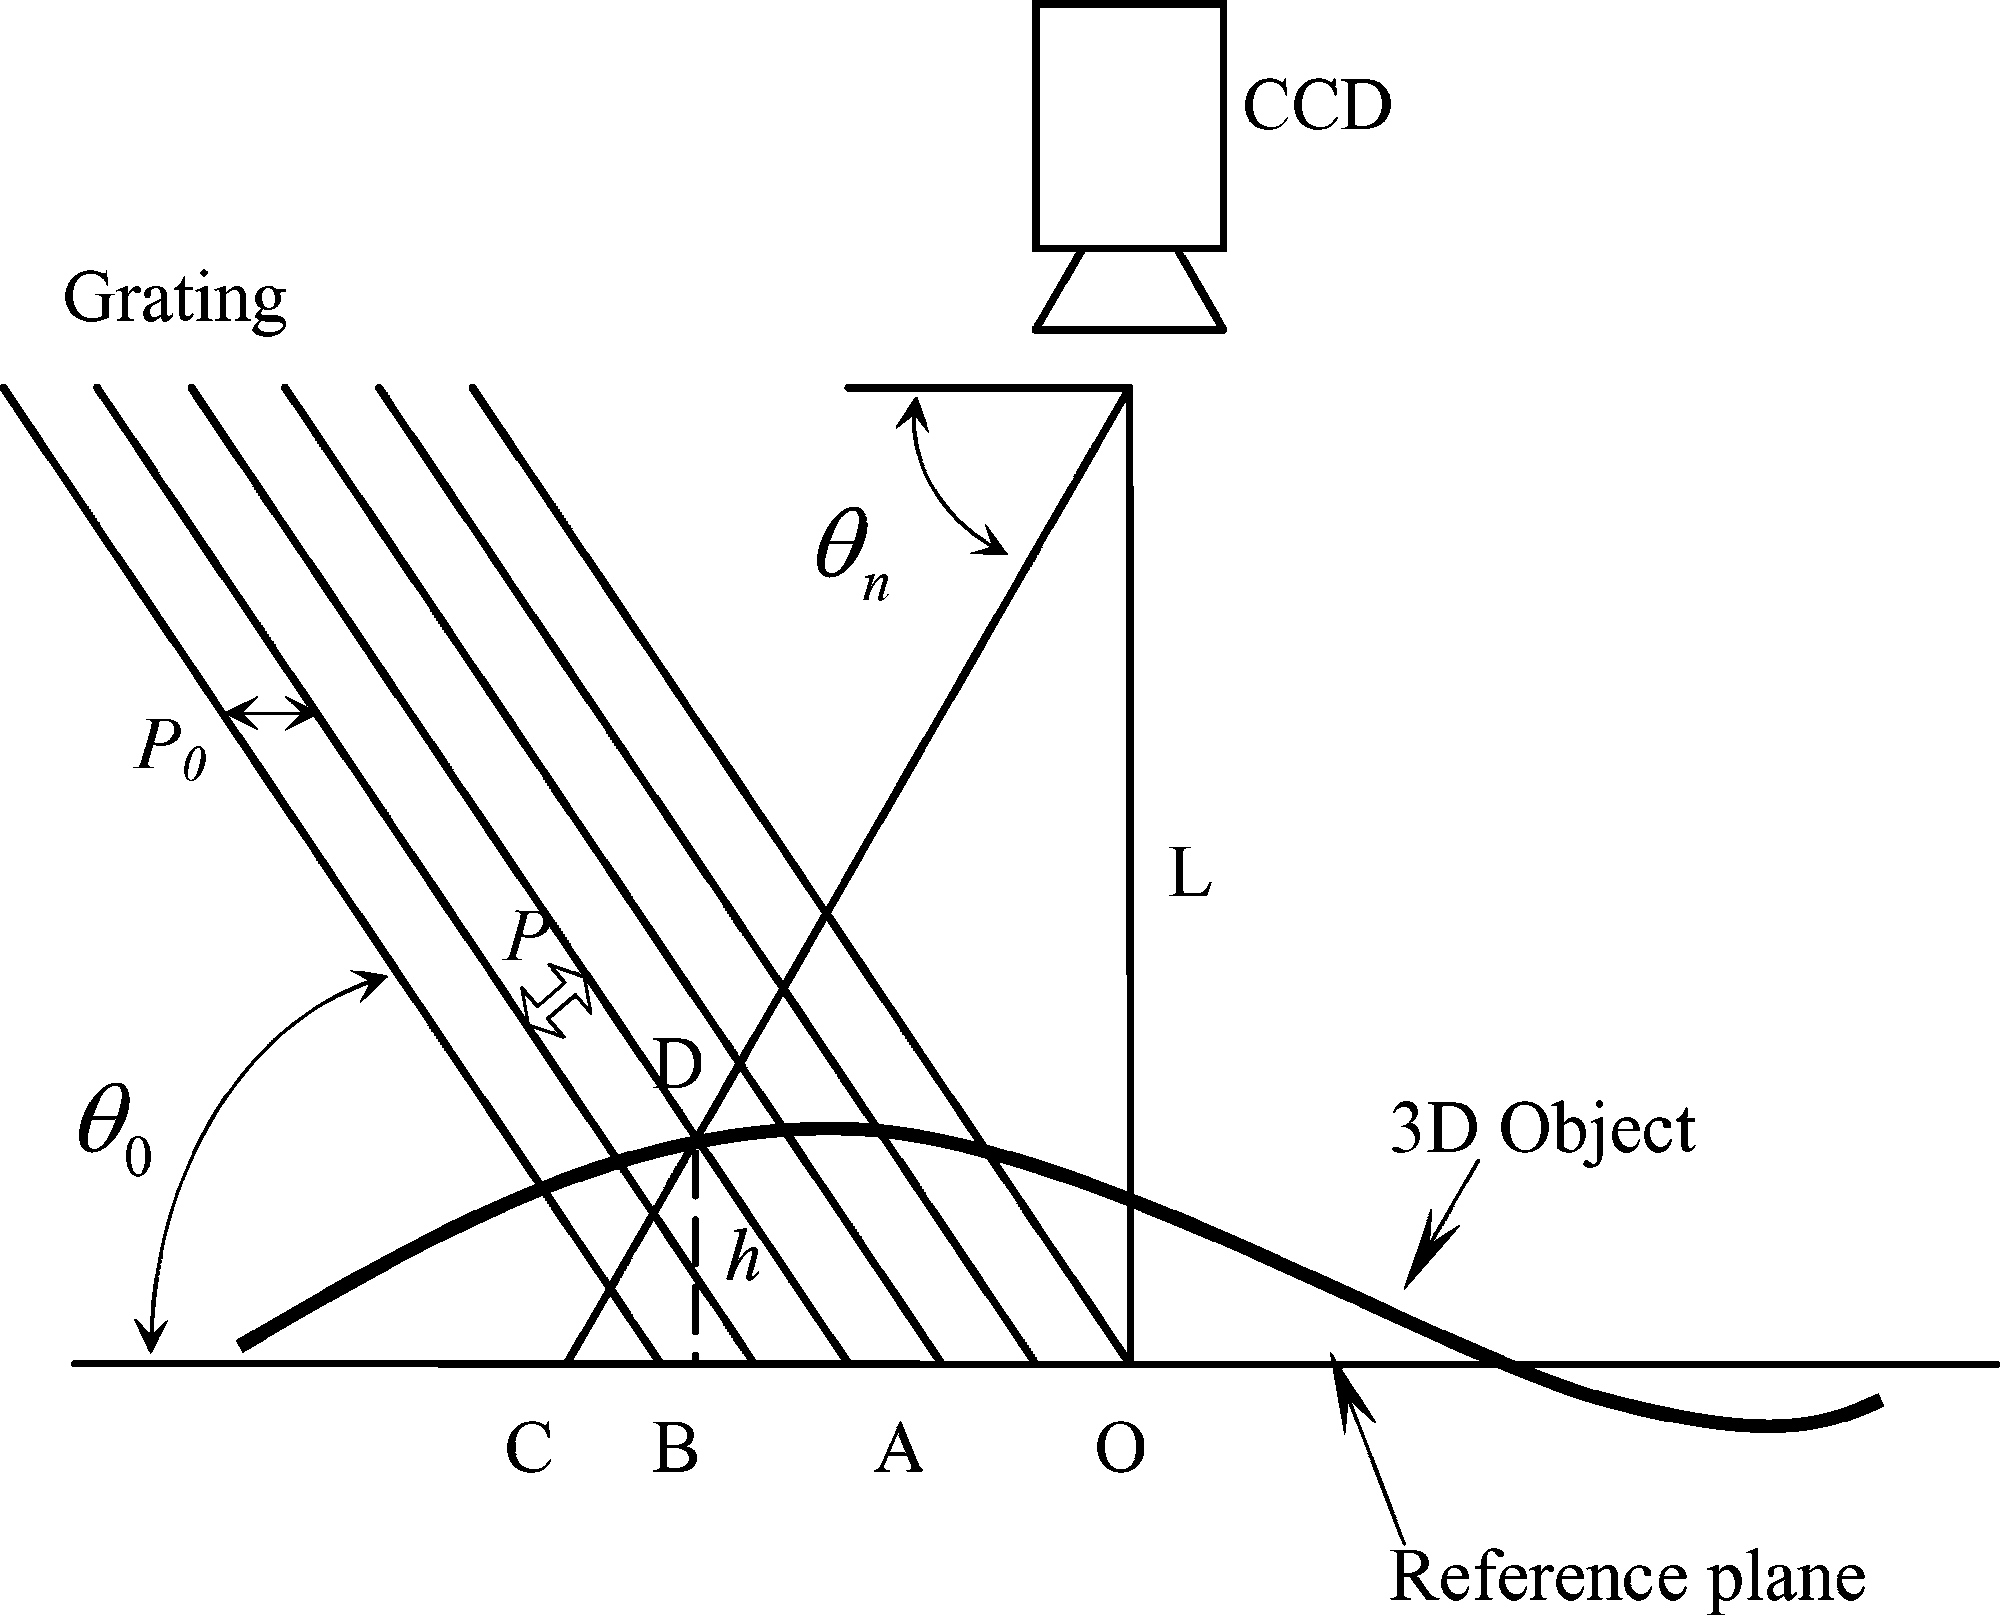
\includegraphics[width=0.9\linewidth]{ch-pastwork/figures/sli}
    \caption[The principle of structured-light imaging]{The principle of structured-light imaging\cite{Li:2009eq}}
    \label{fig:pastwork:sli}
  \end{center}
\end{figure}

Although many other variants of structured light projection are possible, patterns of parallel stripes are widely used. Figure~\ref{fig:pastwork:strippattern} shows the geometrical deformation of a strip pattern projected onto a palm. The displacement of the stripes allows for an exact retrieval of the 3D coordinates of any details on the palm's surface.

David et. al designed a 3D palmprint capturing device~\cite{Zhang:2008kc}. The system proposed has a resolution of 768x576.

\begin{figure}[htb]
  \begin{center}
    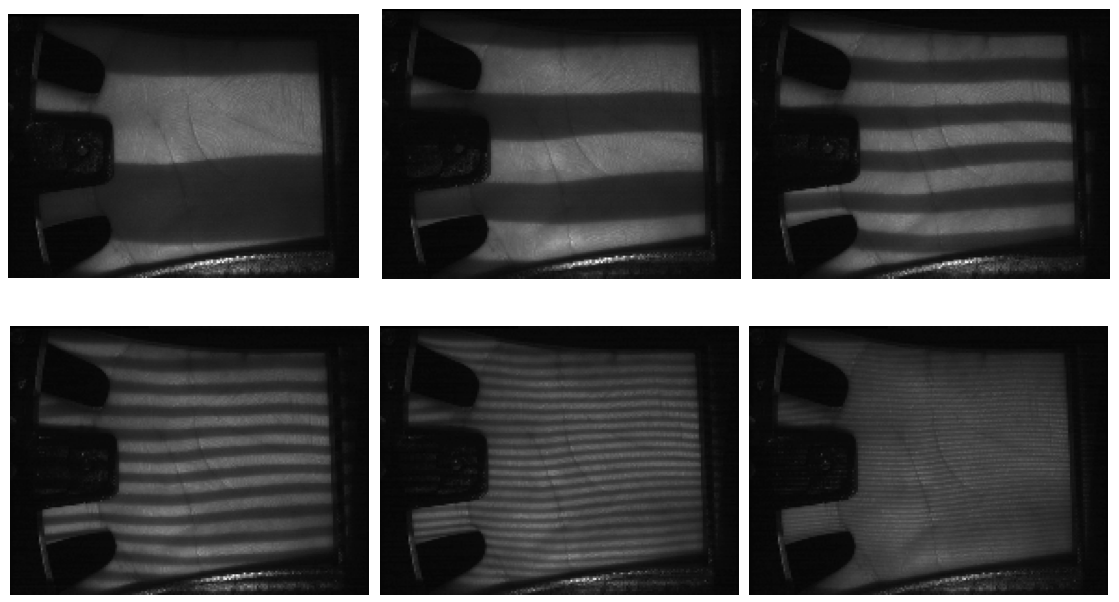
\includegraphics[width=0.9\linewidth]{ch-pastwork/figures/strippattern}
    \caption[Sample patterns of the stripes on the palm]{Sample patterns of the stripes on the palm~\cite{Li:2009eq}}
    \label{fig:pastwork:strippattern}
  \end{center}
\end{figure}

\section{Recognition Methods}
\label{sec:pastwork:recogmethods}

Traditionally, palmprint recognition has made use of either high or low resolution 2D palmprint images. High resolution images are suitable for forensic applications [3] while low resolution images are suitable for civil and commercial applications [4]. Most current research use low resolution palmprint recognition and is either texture-based or line-based. The texture-based methods include PalmCode [4], Competitive Code [5] and Ordinal Code [6]. These methods use a group of filters to enhance and extract the phase or directional features which can represent the texture of the palmprint. Line-based methods use line or edge detectors to explicitly extract line information from the palmprint that is then used for matching. The representative methods include Derivative of Gaussian based line extraction [7] and Modified Finite Radon transform (MFRAT) based line extraction [8].

In recent years, 3D techniques have been applied to biometric authentication, such as 3D face [9] and 3D ear recognition [10]. Most recently, a structured-light imaging [11, 12] 3D palmprint system [13] was developed that captures the depth information of a palmprint. This information is then used to calculate the Mean and the Gaussian curvatures for use in 3D palmprint matching and recognition. To date, however, there has been no work with 3D palmprints that has extracted global shape features, which may be useful in classification and indexing. For fingerprint, according to the global ridge structure and singularities, it can be classified into five classes: arch, tented arch, left loop, right loop and whorl [14]. Wu et al. classified the palmprint into six classes according to the palmprint principal lines [15]. Besides the exclusive classification technique, the continuous classification technique is also widely used for indexing the database for personal identification [16].

Some general features were extracted for recognition including 3D Mean Curvature Image, 3D Gauss Curvature Image and 3D Surface Type~\cite{Zhang:2008kc,Li:2009eq}.




%!TEX root = ../thesis.tex
\chapter{Recognition Procedure\label{ch:methodology}}

The process for feature extraction and matching are described in the following sections in the exact order they are applied to samples in the database.

%!TEX root = chapter-methodology.tex
\section{Region of Interest Extraction}
\label{sec:methodology:roiextraction}

The raw 3D palmprint image consists of 768*576 pixels with a depth value at each point. The samples are captured by a 3D palmprint acquisition device based on structured light imaging ~\cite{Zhang:2009dp}. Before any other processing, noisy pixels at the boundaries must be removed. The full resolution sample is cropped to a Region of Interest (ROI) with 400*400 resolution. A rectangle mask, from (234,68) to (634,468) is used to crop the ROI. Figure ~\ref{fig:methodology:sample-fullres} shows a full resolution sample of a palmprint and Figure ~\ref{fig:methodology:sample-roi} shows the ROI cropped. To reduce the storage and computation requirements for further processing, the ROI is down-sampled to a resolution of 200*200.

\begin{figure}[htb]
  \begin{center}
    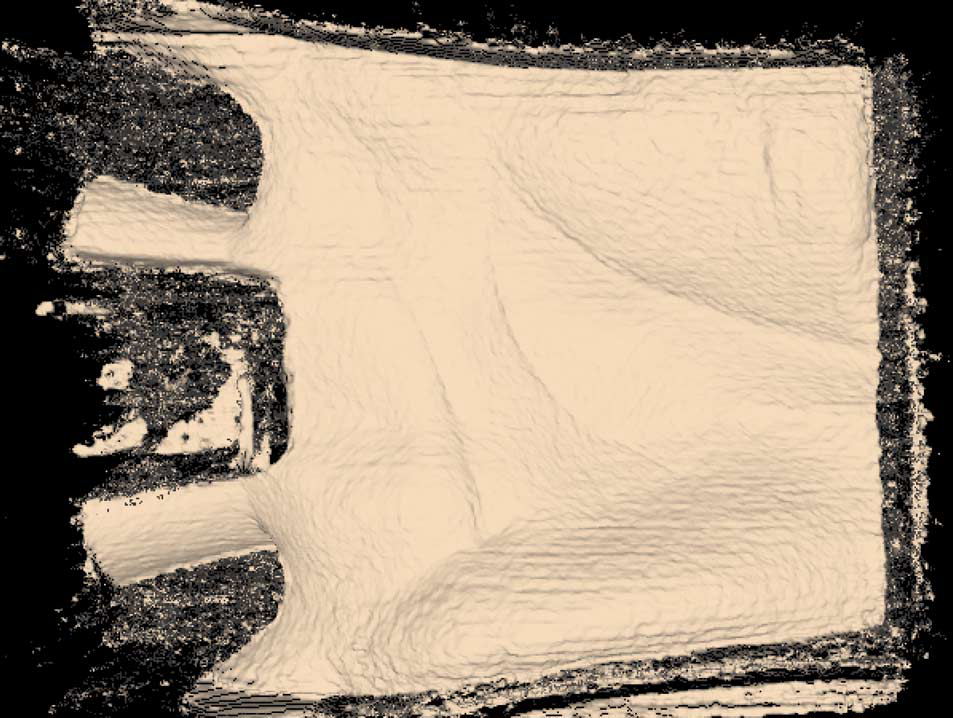
\includegraphics[width=0.9\linewidth]{ch-methodology/figures/sample-fullres}
    \caption[Full resolution 3-D palmprint sample]{Full resolution 3-D palmprint sample}    \label{fig:methodology:sample-fullres}
  \end{center}
\end{figure}

\begin{figure}[htb]
  \begin{center}
    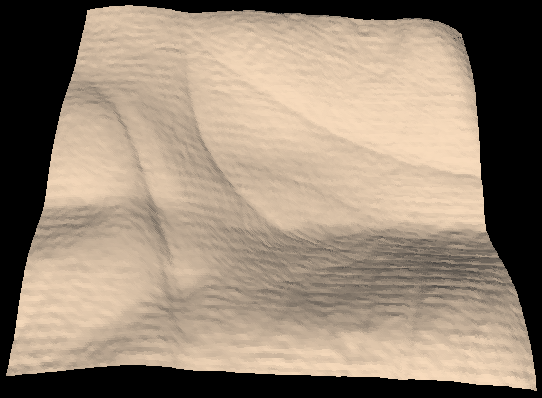
\includegraphics[width=0.9\linewidth]{ch-methodology/figures/sample-roi}
    \caption[ROI from a 3-D palmprint sample]{ROI from a 3-D palmprint sample}
    \label{fig:methodology:sample-roi}
  \end{center}
\end{figure}

The ROI data is stored in a 200 by 200 matrix,

\begin{equation}
\label{eq:methodology:roimatrix}
D=d_{ij}|i=1,2,\dots,200; j=1,2,\dots,200
\end{equation}

where $d_{ij}$ is the depth value of the $i^{th}$ row and $j^{th}$ column pixel of the ROI.

%TODO find the citation
There exists more complicated ROI extraction methods taking advantage of the 2D approaches. 2D ROI is first obtained using the algorithm in ~\cite{Zhang:2003uf}. As the 2D sample captured is pixel-to-pixel matched to the 3D sample, using the exact 2D ROI for the 3D sample is trivial.

The cropping ROI extraction approach used here is much easier and faster than the one proposed in [4]. The reason to adopt this naive approach is that the features are invariant to rotation and translation. It is unnecessary to fully align every sample. Another consideration is that when the 3D information is the only data available, it is not feasible to apply the same 2D algorithm to the depth image.

Even if the samples are cropped to the center area, it is still possible that some noisy pixels are included. If the gradient

\begin{equation}
|\nabla D|=\sqrt{
\left(\frac{\partial{D}}{\partial{x}}\right)^2 +
\left(\frac{\partial{D}}{\partial{y}}\right)^2
}
\end{equation}

is larger than a given threshold, the pixel is regarded as noisy. Another 200 by 200 matrix,

\begin{equation}
\label{eq:methodology:roimask}
M=m_{ij}|i=1,2,\dots,200;j=1,2,\dots,200
\end{equation}

is used to represent the mask, where $m_{ij}=0$ marks the noisy pixels while $m_{ij}=1$ marks the normal ones.
\section{Feature Calculation}
\label{sec:methodology:featurecalc}

Using the ROI obtained from the original 3D palmprint data, three kinds of features to describe the shape of the 3D palmprint: Maximum Depth (MD) of palm center, the Horizontal Cross-section Area (HCA) of different levels and the Radial Line Length (RLL) from the centroid to the boundary of 3D palmprint horizontal cross-section of different levels.

%!TEX root = featurecalc.tex
\subsection{Maximum Depth (MD)}
\label{ssec:methodology:md}

MD means the maximum depth value of the 3D palm from a reference plane. The reference plane is decided using a rectangle obtained by experience. The top left and bottom right pixels of the rectangle are (65,6) and (136,35). These parameters are denoted as $R_s=65, R_e=136, C_s=6$ and $C_e=35$, i.e. the starting(ending) row(column). By examine a random 20 samples, gradient of this area is relatively small.

The depth of the reference plane is defined as the mean depth of the points contained by this rectangle

\begin{equation}
d_r = {1\over{
\sum \limits_{i=R_s}^{R_e} \sum \limits_{j=C_s}^{C_e} m_{ij}
}}
\sum \limits_{i=R_s}^{R_e} \sum \limits_{j=C_s}^{C_e} (d_{ij} \cdot d_{ij})
\end{equation}

where $d_{ij}$ and $m_{ij}$ are the elements defined in ~\ref{eq:methodology:roimatrix} and ~\ref{eq:methodology:roimask}

After getting the depth of the reference plane, we find the maximum depth $d_{max}$ in another region with $R_s=41, R_e=160, C_s=65$ and $C_e=190$.

\begin{equation}
d_{max} = \max \limits_{i=R_s}^{R_e} (\max \limits_{j=C_s}^{C_e} (d_{ij}) )
\end{equation}


The Maximum Depth (MD) is then defined as

\begin{equation}
\label{eq:methodology:md}
MD= d_{max} - d_r
\end{equation}
%!TEX root = featurecalc.tex
\subsection{Horizontal Cross-section Area}
\label{ssec:methodology:hca}

When 3D ROI is examined in a contour view as shown in Figure ~\ref{fig:methodology:roicontour}, it is obvious that the regions of different given depth ranges can be used to describe a sample.

\begin{figure}[htb]
\begin{center}
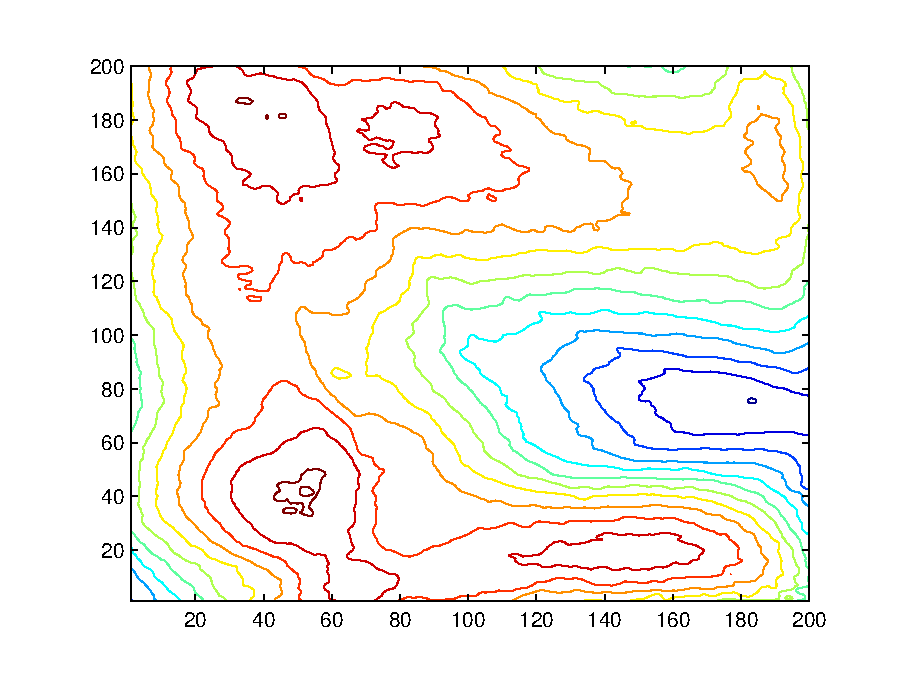
\includegraphics[width=0.9\linewidth]{ch-methodology/figures/roicontour}
\caption[Contour view of a 3D ROI]{Contour view of a 3D ROI}
\label{fig:methodology:roicontour}
\end{center}
\end{figure}

A group of equidistant horizontal planes cut the 3D ROI as shown in Figure ~\ref{fig:methodology:planecut}. Figure ~\ref{fig:methodology:roicontour} shows that most of the deeper level (enclosed with blue curves) are connected. These are more stable in response to noise or transformation.

\begin{figure}[htb]
\begin{center}
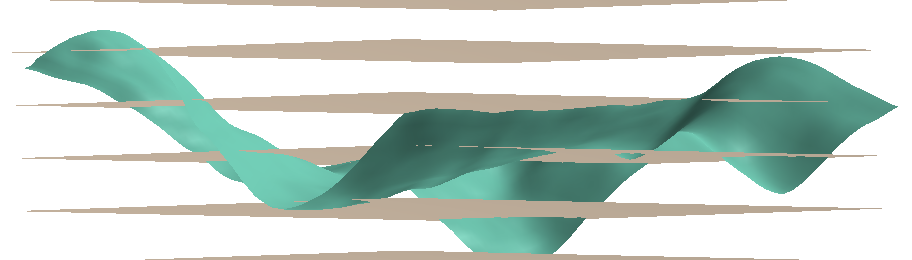
\includegraphics[width=0.9\linewidth]{ch-methodology/figures/planecut}
\caption[3D ROI cut by parallel horizontal planes]{3D ROI cut by parallel horizontal planes}
\label{fig:methodology:planecut}
\end{center}
\end{figure}


To get a stable HCA, we take into consideration only the levels from the deepest point to the reference plane, defined in Section ~\ref{ssec:methodology:md}. Suppose we divide this region into $N$ levels. Every level $G^k, k=1,2,\dots,N$ is described with a 200 by 200 matrix and calculated as

\begin{equation}
G^k_{ij} =
\begin{cases}
1 & \text{if } d_{ij}>h\cdot(N-k+1)/N,\\
0 & \text{otherwise}
\end{cases}
k=1,2,\dots,N;i=1,2,\dots,200;j=1,2,\dots,200;
\end{equation}

where $d_{ij}$ is the depth value of the $i^{th}$ row and $j^{th}$ column pixel of the ROI defined in ~\ref{eq:methodology:roimatrix} and $h$ is the palmprint depth defined by ~\ref{eq:methodology:md}.

To stabilize the areas, the growth of higher level is constrained to its previous level except the first level. That is

\begin{equation}
L^k=
\begin{cases}
G^1                             & k=1 \\
G^k \cap (L^{k-1} \oplus \Theta^{k-1}) & k=2,3,\dots,N
\end{cases}
\end{equation}

where $\cap$ denotes logical AND, $\oplus$ denotes a morphological dilation operation and  $\Theta^{k}$ is a disk morphological structuring element whose size can be calculated by $35-3 \times k$ (which is suitable for N = 8 by experience).

\begin{figure}[htb]
\begin{center}
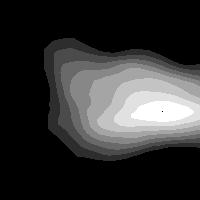
\includegraphics[width=0.9\linewidth]{ch-methodology/figures/hcastack}
\caption[$L^k$ shown stacked when $N=8$]{$L^k$ shown stacked when $N=8$}
\label{fig:methodology:hcastack}
\end{center}
\end{figure}

Figure ~\ref{fig:methodology:hcastack} shows an example of all the levels stacked together.

\begin{figure}[htb]
\centering
\subfigure[$k=1$]{
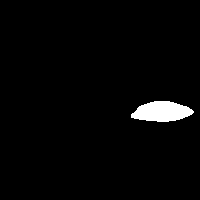
\includegraphics[height=0.18\textheight]{ch-methodology/figures/hca1-1}
\label{fig:methodology:hcalevels:1-1}
}\hspace{0.15\linewidth}
\subfigure[$k=2$]{
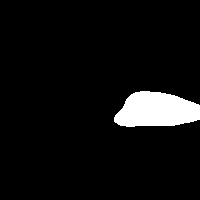
\includegraphics[height=0.18\textheight]{ch-methodology/figures/hca1-2}
\label{fig:methodology:hcalevels:1-2}
}\\
\subfigure[$k=3$]{
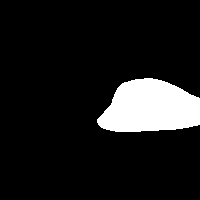
\includegraphics[height=0.18\textheight]{ch-methodology/figures/hca1-3}
\label{fig:methodology:hcalevels:1-3}
}\hspace{0.15\linewidth}
\subfigure[$k=4$]{
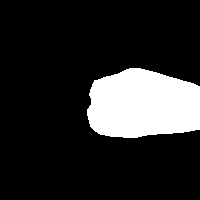
\includegraphics[height=0.18\textheight]{ch-methodology/figures/hca1-4}
\label{fig:methodology:hcalevels:1-4}
}\\
\subfigure[$k=5$]{
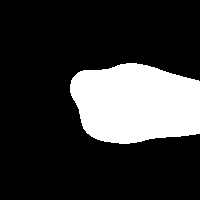
\includegraphics[height=0.18\textheight]{ch-methodology/figures/hca1-5}
\label{fig:methodology:hcalevels:1-5}
}\hspace{0.15\linewidth}
\subfigure[$k=6$]{
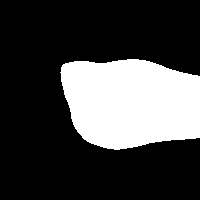
\includegraphics[height=0.18\textheight]{ch-methodology/figures/hca1-6}
\label{fig:methodology:hcalevels:1-6}
}\\
\subfigure[$k=7$]{
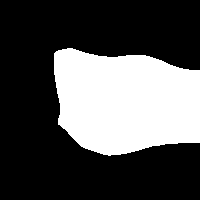
\includegraphics[height=0.18\textheight]{ch-methodology/figures/hca1-7}
\label{fig:methodology:hcalevels:1-7}
}\hspace{0.15\linewidth}
\subfigure[$k=8$]{
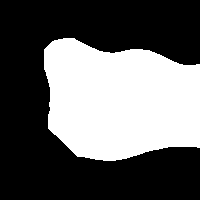
\includegraphics[height=0.18\textheight]{ch-methodology/figures/hca1-8}
\label{fig:methodology:hcalevels:1-8}
}
\caption[$L^k$ of one sample from palm 1]{$L^k$ for $k=1,2,\dots,8$ of a 3D ROI from a palmprint sample}
\label{fig:methodology:hcalevels1}
\end{figure}


\begin{figure}[htb]
\centering
\subfigure[$k=1$]{
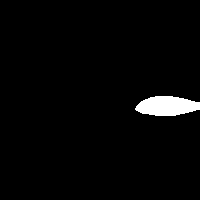
\includegraphics[height=0.18\textheight]{ch-methodology/figures/hca2-1}
}\hspace{0.15\linewidth}
\subfigure[$k=2$]{
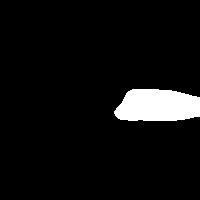
\includegraphics[height=0.18\textheight]{ch-methodology/figures/hca2-2}
}\\
\subfigure[$k=3$]{
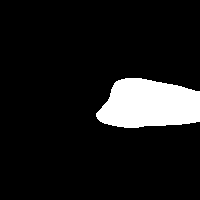
\includegraphics[height=0.18\textheight]{ch-methodology/figures/hca2-3}
}\hspace{0.15\linewidth}
\subfigure[$k=4$]{
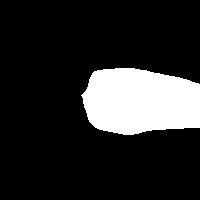
\includegraphics[height=0.18\textheight]{ch-methodology/figures/hca2-4}
}\\
\subfigure[$k=5$]{
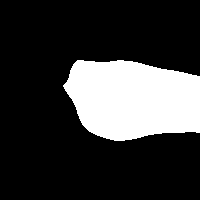
\includegraphics[height=0.18\textheight]{ch-methodology/figures/hca2-5}
}\hspace{0.15\linewidth}
\subfigure[$k=6$]{
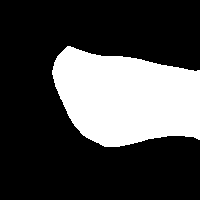
\includegraphics[height=0.18\textheight]{ch-methodology/figures/hca2-6}
}\\
\subfigure[$k=7$]{
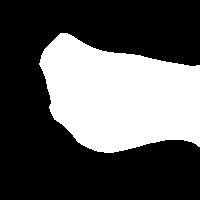
\includegraphics[height=0.18\textheight]{ch-methodology/figures/hca2-7}
}\hspace{0.15\linewidth}
\subfigure[$k=8$]{
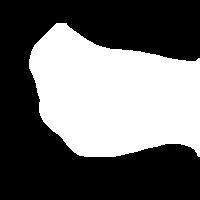
\includegraphics[height=0.18\textheight]{ch-methodology/figures/hca2-8}
}
\caption[$L^k$ of another sample from palm 1]{$L^k$ for $k=1,2,\dots,8$ of a 3D ROI from another palmprint sample from the same person as in Figure ~\ref{fig:methodology:hcalevels1}}
\label{fig:methodology:hcalevels2}
\end{figure}

\begin{figure}[htb]
\centering
\subfigure[$k=1$]{
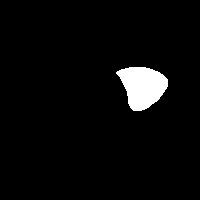
\includegraphics[height=0.18\textheight]{ch-methodology/figures/hca3-1}
}\hspace{0.15\linewidth}
\subfigure[$k=2$]{

\includegraphics[height=0.18\textheight]{ch-methodology/figures/hca3-2}
}\\
\subfigure[$k=3$]{

\includegraphics[height=0.18\textheight]{ch-methodology/figures/hca3-3}
}\hspace{0.15\linewidth}
\subfigure[$k=4$]{
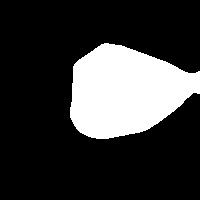
\includegraphics[height=0.18\textheight]{ch-methodology/figures/hca3-4}
}\\
\subfigure[$k=5$]{
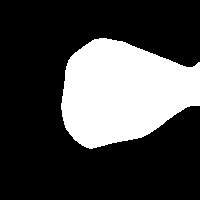
\includegraphics[height=0.18\textheight]{ch-methodology/figures/hca3-5}
}\hspace{0.15\linewidth}
\subfigure[$k=6$]{
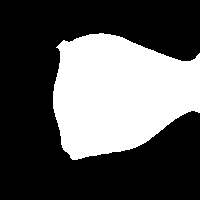
\includegraphics[height=0.18\textheight]{ch-methodology/figures/hca3-6}
}\\
\subfigure[$k=7$]{
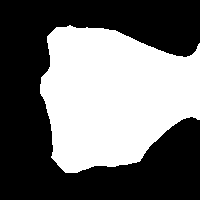
\includegraphics[height=0.18\textheight]{ch-methodology/figures/hca3-7}
}\hspace{0.15\linewidth}
\subfigure[$k=8$]{
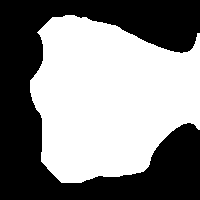
\includegraphics[height=0.18\textheight]{ch-methodology/figures/hca3-8}
}
\caption[$L^k$ of one sample from palm 2]{$L^k$ for $k=1,2,\dots,8$ of a 3D ROI from a palmprint sample from the a different person from that of Figure ~\ref{fig:methodology:hcalevels1}}
\label{fig:methodology:hcalevels3}
\end{figure}

\begin{figure}[htb]
\centering
\subfigure[$k=1$]{

\includegraphics[height=0.18\textheight]{ch-methodology/figures/hca4-1}
}\hspace{0.15\linewidth}
\subfigure[$k=2$]{

\includegraphics[height=0.18\textheight]{ch-methodology/figures/hca4-2}
}\\
\subfigure[$k=3$]{
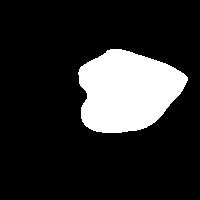
\includegraphics[height=0.18\textheight]{ch-methodology/figures/hca4-3}
}\hspace{0.15\linewidth}
\subfigure[$k=4$]{
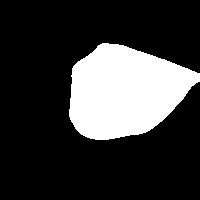
\includegraphics[height=0.18\textheight]{ch-methodology/figures/hca4-4}
}\\
\subfigure[$k=5$]{
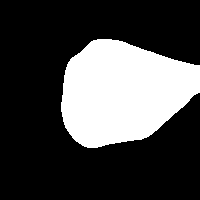
\includegraphics[height=0.18\textheight]{ch-methodology/figures/hca4-5}
}\hspace{0.15\linewidth}
\subfigure[$k=6$]{
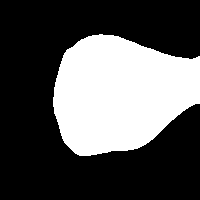
\includegraphics[height=0.18\textheight]{ch-methodology/figures/hca4-6}
}\\
\subfigure[$k=7$]{
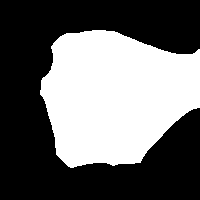
\includegraphics[height=0.18\textheight]{ch-methodology/figures/hca4-7}
}\hspace{0.15\linewidth}
\subfigure[$k=8$]{
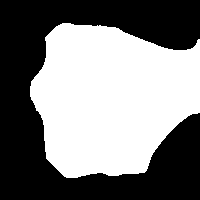
\includegraphics[height=0.18\textheight]{ch-methodology/figures/hca4-8}
}
\caption[$L^k$ of another sample from palm 2]{$L^k$ for $k=1,2,\dots,8$ of a 3D ROI from another palmprint sample from the same person as in Figure ~\ref{fig:methodology:hcalevels3}}
\label{fig:methodology:hcalevels4}
\end{figure}

Figure ~\ref{fig:methodology:hcalevels1} and ~\ref{fig:methodology:hcalevels2} shows the cross-sectional area feature from two samples collected from one palm. Figure ~\ref{fig:methodology:hcalevels3} and ~\ref{fig:methodology:hcalevels4} are extracted from two samples from another palm.

\subsection{Radial Line Length (RLL)}
\label{ssec:methodology:rll}

HCA is a coarse summary of the ROI characteristics. Different sample may have a similar area but dramatically different shape or contour of that area. To describe this shape characteristic, we need more elements to represent the ROI. The Radial Line Length (RLL) is then introduced for this purpose.

First, we calculate the centroid of the first level  $L^1$, thereafter we treat it as the reference point $P_{ref}$ for all levels. Then, from $P_{ref}$ we draw M radial lines which intersect with the contour of every level. RLL is defined as the distance from the intersection point to $P_{ref}$. The radial lines are distributed at equal angles. We record these radial lines from the inner layers to the outer layers starting with the horizontal direction by an $M$ by $N$ dimensional vector
\begin{equation}
R_i, i=1,2,\dots,M\times N
\end{equation}
where $M$ is the number of radial lines and $N$ is the number of cross-sections.

Figure ~\ref{fig:methodology:rll8} through ~\ref{fig:methodology:rll64} show some examples of RLL. This is a more detailed description than HCA as it takes the shape of each area into consideration.

\begin{figure}[htb]
  \begin{center}
    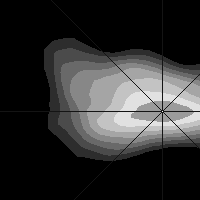
\includegraphics[width=0.4\linewidth]{ch-methodology/figures/rll8}
    \caption[8 radial lines starting from the reference point]{8 radial lines starting from the reference point}
    \label{fig:methodology:rll8}
  \end{center}
\end{figure}

\begin{figure}[htb]
  \begin{center}
    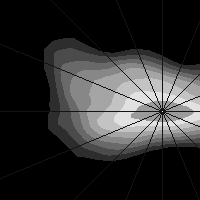
\includegraphics[width=0.4\linewidth]{ch-methodology/figures/rll16}
    \caption[16 radial lines starting from the reference point]{16 radial lines starting from the reference point}
    \label{fig:methodology:rll16}
  \end{center}
\end{figure}

\begin{figure}[htb]
  \begin{center}
    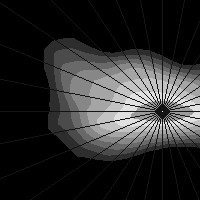
\includegraphics[width=0.4\linewidth]{ch-methodology/figures/rll32}
    \caption[32 radial lines starting from the reference point]{32 radial lines starting from the reference point}
    \label{fig:methodology:rll32}
  \end{center}
\end{figure}

\begin{figure}[htb]
  \begin{center}
    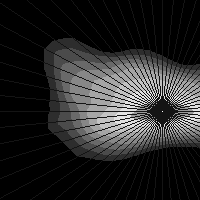
\includegraphics[width=0.4\linewidth]{ch-methodology/figures/rll64}
    \caption[64 radial lines starting from the reference point]{64 radial lines starting from the reference point}
    \label{fig:methodology:rll64}
  \end{center}
\end{figure}



The above three features are mainly determined by the central region of the palm. This region is certainly contained by the ROI described in Section ~\ref{sec:methodology:roiextraction} which makes these features insensitive to translation and rotation. Although the RLL feature can be affected by rotation as the contours change smoothly, if the rotation is small then the variation of the RLL feature will also be small. Actually, there are some restricting pegs on the capture device which can guide the users to put their hands on the proper place as described in ~\cite{Zhang:2009dp}. Furthermore, we assume the user is cooperative when collecting data as we aim at civil rather than law enforcement applications.

%!TEX root = chapter-methodology.tex
\section{Feature Matching}
\label{sec:methodology:featurematch}

%TODO find the citaions
The classification of biometrics speeds up the identification process by reducing the number of comparisons that must be made. There are two kinds of classification techniques: exclusive classification and continuous classification. Both fingerprint ~\cite{Henry:1900vc} and palmprint classifications ~\cite{Wu:2004kx} make use of exclusive classification. The main problem of this technique is that it uses only a small number of classes and the samples are unevenly distributed between them, with more than 90\% of the samples being in just two or three classes. A further problem with exclusive classification is that when classification is performed automatically, it is necessary to handle errors and rejected samples gracefully, which is a hard problem in practice. In contrast, for continuous classification, samples are not partitioned into disjoint classes but rather associated with numerical vectors which represent features of the samples. These feature vectors are created through a similarity-preserving transformation so that similar samples are mapped into close points in the multi-dimensional space ~\cite{Maltoni:wn}. The continuous classification technique is adopted. As the features combining MD, HCA and RLL are high-dimensional, LDA is used for dimension reduction. Coarse-level matching and Ranking Support Vector Machine (RSVM) are applied to the low dimensional vectors for efficient palmprint recognition.

\subsection{Dimension Reduction}
\label{ssec:methodology:lda}

LDA is a state-of-the-art dimensionality reduction technique widely used in classification problems. The objective is to find the optimal projection which simultaneously minimizes the within-class distance and maximizes the between-class distance, thus achieving maximum discrimination (Here, the “class” is used to denote the identity of the subjects, e.g. the samples collected from one palm are regarded as one class). However, the traditional LDA requires the within-class scatter matrix to be nonsingular, which means the sample size should be large enough compared with its dimension, but is not always possible. In this paper, we therefore adopt the orthogonal LDA (OLDA) proposed in [17], where the vectors of the optimal projection are calculated using the training database and the optimal projecting vectors are orthogonal to each other.
Suppose the 3D ROI has been divided to N levels and that M radial lines are used to represent the level contours. We can list the global features as a column vector,  , with   rows. Given a training database which has n samples and k classes as  , where   and  , adopting OLDA [17] the optimal projection W can be calculated as follows.
First, the within-class scatter matrix  , the between-class scatter matrix   and total scatter matrix   can be expressed as
                              (6)
where
                           (7)
                         (8)
                                         (9)
where   is the centroid of the ith class  ,   is the centroid of all the training samples ,   and  .
After calculating  ,   and  , the reduced Singular Value Decomposition (SVD) is applied to  .
                                     (10)
Denote   and compute the SVD of B.
                                          (11)
Let
                                              (12)
                                              (13)
and denote   the first   columns of the matrix D. Then, compute the QR decomposition of  .
                                    (14)
where Q is the desired orthogonal matrix and optimal projection, i.e.  .
After getting the optimal projection W, we can map the   dimensional vector F to a lower dimensional space
                                             (15)
where   is a   dimensional vector with  .

%!TEX root = featurematch.tex
\subsection{Coarse-level Matching}
\label{ssec:methodology:naive}

For palmprint recognition, we need a measurement of similarity between two samples. If the similarity is high, we have a high confidence to believe that the two samples are from the same person. Otherwise we reject to claim that.

After mapping the high-dimensional feature vector to $\Gamma$-dimensional vector $\tilde{F}$, the similarity between two samples can be calculated as

\begin{equation}
Similarity= \| \tilde{F}_1 -\tilde{F}_2 \|
= \sum \limits_{i=1}^{\Gamma} (f_i^1-f_i^2)^2
\label{eq:methodology:similarity}
\end{equation}

\begin{figure}[htb]
  \begin{center}
    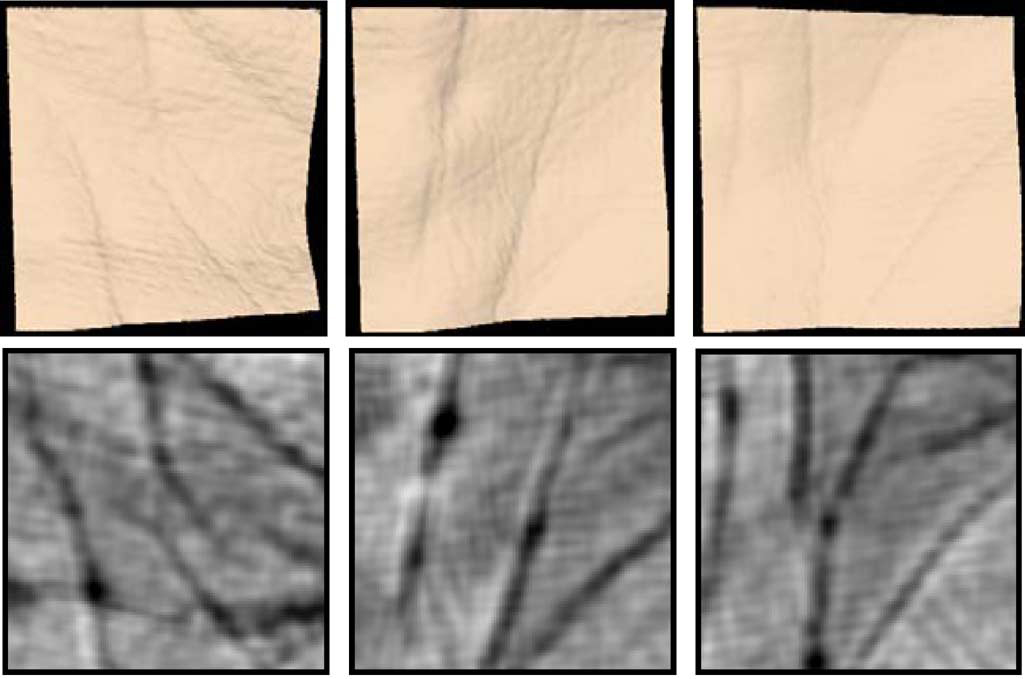
\includegraphics[width=0.9\linewidth]{ch-methodology/figures/mci1}
    \caption[MCI for ROIs from different palms]{Mean Curvature Image for ROIs from three different palms}    \label{fig:methodology:mci1}
  \end{center}
\end{figure}

\begin{figure}[htb]
  \begin{center}
    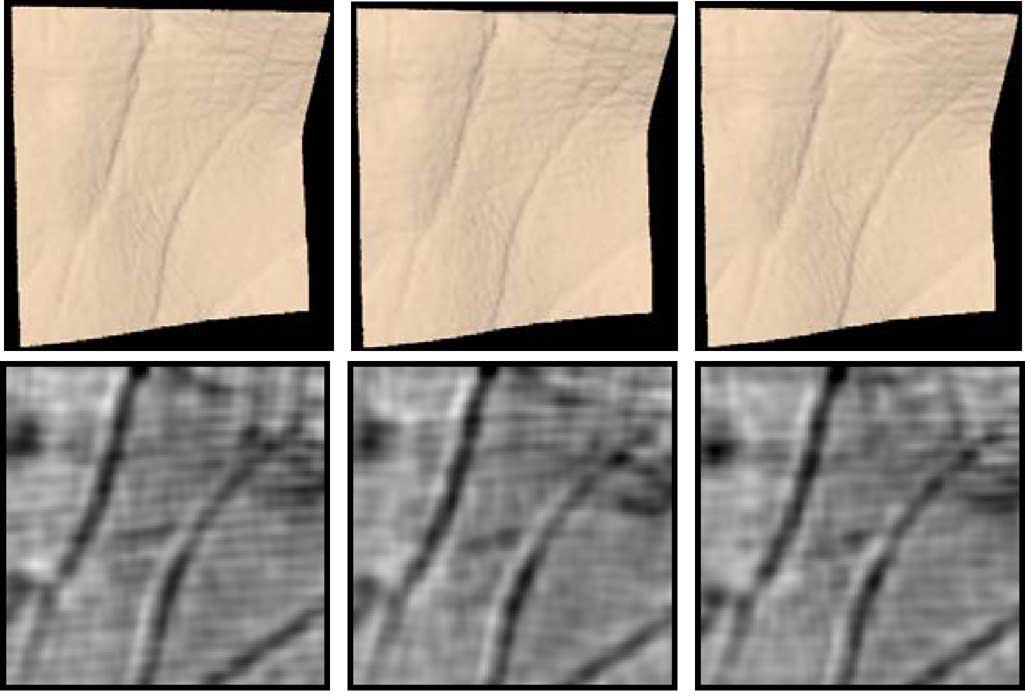
\includegraphics[width=0.9\linewidth]{ch-methodology/figures/mci2}
    \caption[MCI for ROIs from the same palm]{Mean Curvature Image for ROIs from three samples of the same palm}    \label{fig:methodology:mci2}
  \end{center}
\end{figure}

There are other features extracted from the same dataset such as Mean Curvature Image in ~\cite{Zhang:2009dp}. Figure ~\ref{fig:methodology:mci1} shows the ROI and MCI extracted from three different palms while Figure ~\ref{fig:methodology:mci2} show samples from the same palm. The corresponding matching score is defined as

\begin{equation}
Y=\frac{
    2\sum \limits_{i=1}^{n} \sum \limits_{j=1}^{m} Z_d(i,j) \cap Z_t(i,j)
}
{
    \sum \limits_{i=1}^{n} \sum \limits_{j=1}^{m} Z_d(i,j) +
    \sum \limits_{i=1}^{n} \sum \limits_{j=1}^{m} Z_t(i,j)
}
\end{equation}

where symbol $\cap$ represents the logical AND operation, $Z_d$ and $Z_t$ are two binarized MCIs. Due to the fact that MCI is covariant to shifting, the actual matching process for MCI is repeated by shifting the image with 4 different displacement in 8 directions. A total of 33 matching scores are calculated and the maximum is adopted as the overall matching score.

Although MCI feature is more descriptive, it takes up more storage ($200\times200$ floats to store the feature image). Compared to the computation in ~\ref{eq:methodology:similarity}, the MCI matching process requires far more computation and is therefore significantly slower.
% Table generated by Excel2LaTeX from sheet 'Sheet1'
\begin{table}[htbp]
  \centering
  \caption{Penetration rate and error rate using RSVM}
    \begin{tabular}{|c|c|}
    \hline
    Penetration rate (\%) & Error rate (\%) \\
    \hline
    30    & 1.3 \\ \hline
    27.5  & 1.33 \\ \hline
    25    & 1.37 \\ \hline
    22.5  & 1.42 \\ \hline
    20    & 1.49 \\ \hline
    17.5  & 1.63 \\ \hline
    15    & 1.87 \\ \hline
    12.5  & 2.48 \\ \hline
    10    & 3.35 \\ \hline
    7.5   & 4.41 \\ \hline
    5     & 5.88 \\
    \hline
    \end{tabular}%
  \label{tab:experiment:svm}%
\end{table}%



%!TEX root = ../thesis.tex
\chapter{Experimental Results\label{ch:experiment}}

We used the 3D palmprint acquisition device developed in ~\cite{Zhang:2009dp} to establish a 3D palmprint database containing 8000 samples collected from 400 palms. The 3D palmprint samples were collected in two separated sessions, 10 samples in each session. The average time interval between the two sessions is one month. The collection procedure required volunteers to put their palms naturally and without force on the device. As mentioned in Section ~\ref{sec:methodology:roiextraction}, the original spatial resolution of the data was 768×576. After ROI extraction, the central part (400×400) was extracted and downsampled to (200×200) for feature extraction and recognition.

%!TEX root = chapter-experiment.tex
\section{Optimizing Parameters}
\label{sec:experiment:parameters}

The database was divided into a training part (the first session of 4000 samples) and a testing part (the second session of 4000 samples). As described in Section ~\ref{ssec:methodology:lda}, the dimension of the proposed  features is $1+N+N\times M$. To select the value of $M$ and $N$, a series of verifications on the training database were carried out where the class of the input palmprint was known. Each of the 3D samples was matched with the remaining samples in the training database. A successful match is where the two samples are from the same class. This is referred to as intra-class matching and the candidate image is said to be genuine. An unsuccessful match is referred to as inter-class matching and the candidate image is said to be an impostor. Treating the features as a point in the $1+N+N\times M$ dimension space, Euclidian distance is used as the matching score.


%!TEX root = chapter-experiment.tex
\section{Optimizing Parameters}
\label{sec:experiment:parameters}

The database was divided into a training part (the first session of 4000 samples) and a testing part (the second session of 4000 samples). As described in Section ~\ref{ssec:methodology:lda}, the dimension of the proposed  features is $1+N+N\times M$. To select the value of $M$ and $N$, a series of verifications on the training database were carried out where the class of the input palmprint was known. Each of the 3D samples was matched with the remaining samples in the training database. A successful match is where the two samples are from the same class. This is referred to as intra-class matching and the candidate image is said to be genuine. An unsuccessful match is referred to as inter-class matching and the candidate image is said to be an impostor. Treating the features as a point in the $1+N+N\times M$ dimension space, Euclidian distance is used as the matching score.


\input{ch-experiment/tables/parameters}

Table ~\ref{tab:experiment:parameters} shows the Equal Error Rate (EER) for $N=4,8,16$ and $M=8,16,32,64$. The best result, as adopted in Chapter ~\ref{ch:methodology}, is $N=8$ and $M=32$.


In order to balance accuracy and efficiency, we chose $N=8$ and $M=32$ in the following experiments. This means the features have $1+N+N\times M=265$ dimensions.

\input{ch-experiment/tables/verification}

Table ~\ref{tab:experiment:verification} shows the verification results by MD, HCA, RLL and their combined results. From the last column of Table ~\ref{tab:experiment:verification} we can see using the combined three features will achieve a lower EER than each of the individual features.

As described in Section ~\ref{ssec:methodology:lda}, we use the OLDA method to reduce features to a lower dimension $\Gamma$. To decide the optimal value of $\Gamma$, we carried out a series of recognition experiments on the 4000 sample training database. We divided this database into two equal parts and then chose the first five samples of every palm for training and set aside the rest for testing. As shown in Section ~\ref{ssec:methodology:lda}, $\Gamma$ is equal to q in (13). Instead of setting $q=rank(B)$, we set $q=1,2,\dots,10,12,15,20,30$.

\input{ch-experiment/tables/gamma}

Table ~\ref{tab:experiment:gamma} shows the recognition results.

\begin{figure}[htb]
  \begin{center}
    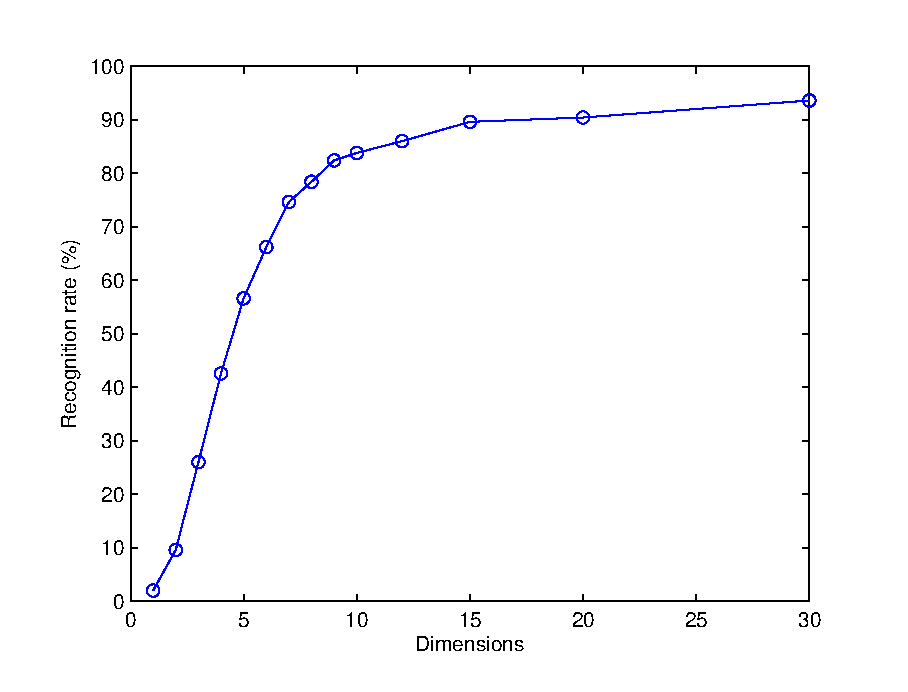
\includegraphics[width=\linewidth]{ch-experiment/figures/gamma}
    \caption[Recognition rate by OLDA for different dimensions]{Recognition rate by OLDA for different dimensions}
    \label{fig:experiment:gamma}
  \end{center}
\end{figure}

According to the curve shown in Figure ~\ref{fig:experiment:gamma}, $\Gamma=15$ is a good choice for the following experiments with balanced recognition rate and computation.

Table ~\ref{tab:experiment:parameters} shows the Equal Error Rate (EER) for $N=4,8,16$ and $M=8,16,32,64$. The best result, as adopted in Chapter ~\ref{ch:methodology}, is $N=8$ and $M=32$.


In order to balance accuracy and efficiency, we chose $N=8$ and $M=32$ in the following experiments. This means the features have $1+N+N\times M=265$ dimensions.

% Table generated by Excel2LaTeX from sheet 'Sheet2'
\begin{table}[htbp]
  \centering
  \caption{The EER of 3D palmprint verification for with each feature and the combined feature}
    \begin{tabular}{ccccc}
    \toprule
    Global features & MD    & HCA   & RLL   & MD+HCA+RLL \\
    \midrule
    EER(\%) & 25.8  & 20.4  & 18.6  & 12.32 \\
    \bottomrule
    \end{tabular}%
  \label{tab:experiment:verification}%
\end{table}%


Table ~\ref{tab:experiment:verification} shows the verification results by MD, HCA, RLL and their combined results. From the last column of Table ~\ref{tab:experiment:verification} we can see using the combined three features will achieve a lower EER than each of the individual features.

As described in Section ~\ref{ssec:methodology:lda}, we use the OLDA method to reduce features to a lower dimension $\Gamma$. To decide the optimal value of $\Gamma$, we carried out a series of recognition experiments on the 4000 sample training database. We divided this database into two equal parts and then chose the first five samples of every palm for training and set aside the rest for testing. As shown in Section ~\ref{ssec:methodology:lda}, $\Gamma$ is equal to q in (13). Instead of setting $q=rank(B)$, we set $q=1,2,\dots,10,12,15,20,30$.

% Table generated by Excel2LaTeX from sheet 'Sheet3'
\begin{table}[htbp]
  \centering
  \caption{Recognition rate by OLDA for different dimensions}
    \tabcolsep=0.11cm
    \begin{tabular}{|r|c|c|c|c|c|c|c|c|c|c|c|c|c|c|}
    \hline
        $\Gamma$  & 1     & 2     & 3     & 4     & 5     & 6     & 7     & 8     & 9     & 10    & 12    & 15    & 20    & 30 \\
    \hline
    Recognition rate (\%) & {2} & {9.6} & {26} & {42.6} & {56.6} & {66.2} & {74.6} & {78.4} & {82.4} & {83.8} & {86} & {89.6} & {90.4} & {93.6} \\
	\hline
    \end{tabular}%
  \label{tab:experiment:gamma}%
\end{table}%


Table ~\ref{tab:experiment:gamma} shows the recognition results.

\begin{figure}[htb]
  \begin{center}
    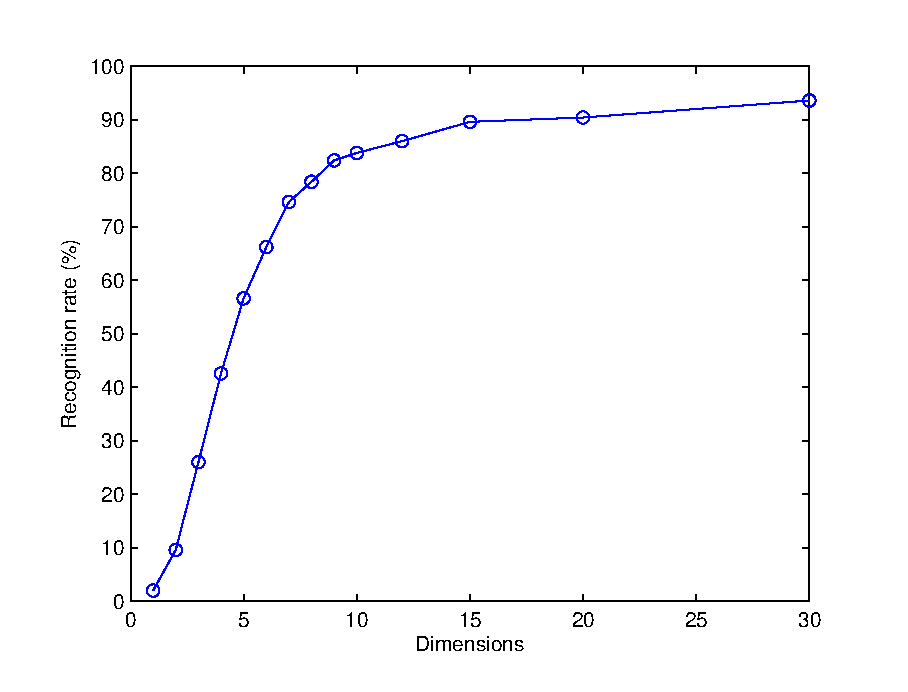
\includegraphics[width=\linewidth]{ch-experiment/figures/gamma}
    \caption[Recognition rate by OLDA for different dimensions]{Recognition rate by OLDA for different dimensions}
    \label{fig:experiment:gamma}
  \end{center}
\end{figure}

According to the curve shown in Figure ~\ref{fig:experiment:gamma}, $\Gamma=15$ is a good choice for the following experiments with balanced recognition rate and computation.
%!TEX root = chapter-experiment.tex
\section{Genuine and Imposter Distributions}
\label{sec:experiment:distribution}

Figure ~\ref{fig:experiment:11p} show the genuine and impostor distributions when the 15-dimensional features are applied to the 4000 training database when calculate the Euclidian distance.

\begin{figure}[htb]
  \begin{center}
    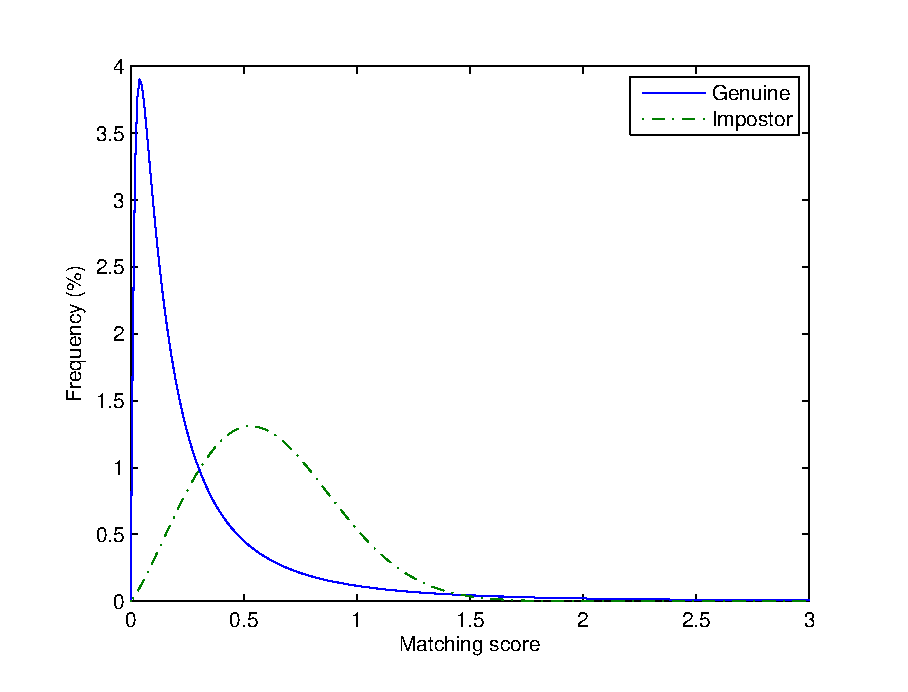
\includegraphics[scale=1]{ch-experiment/figures/11p.eps}
    \caption{Sample distributions by matching the 15-dimensional feature vector}
    \label{fig:experiment:11p}
  \end{center}
\end{figure}


%!TEX root = chapter-experiment.tex
\section{Recognition Performance}
\label{sec:experiment:recognition}

We next carried out the 3D palmprint classification and recognition experiments using the first sample of each class in the training database as a template and the 4000 samples in the testing database as probes, making a total of 400 templates and 4000 probes. The performance of classification and recognition is usually measured by error rate and penetration rate calculated in ~\cite{Maltoni:wn} as follows

\begin{equation}
\text{error rate} = \frac{\text{number of false match}}{\text{total number of probe}} \times 100\%
\end{equation}

\begin{equation}
\text{penetration rate} = \frac{\text{number of accessed template}}{\text{total number of template in the database}} \times 100\%
\label{eq:experiment:prate}
\end{equation}

Obviously there is a trade-off between error rates and penetration rates. Generally speaking, if there is no classification, there are two retrieval strategies:

\begin{enumerate}
\item all of the templates in the database are visited and the template that gives the best matching score is regarded as the matched template, if the matching score is less than a given threshold $\Psi_T$
\item given a threshold $\Psi_T$, the search continues until a match is found that is below that threshold
\end{enumerate}

Three 3D palmprint recognition matching approaches are used

\begin{enumerate}
\item no classification
\item coarse-level matching
\item RSVM
\end{enumerate}

For no classification, we matched using the local feature MCI as described in ~\cite{Zhang:2009dp}. The process we used for coarse-level matching is illustrated in Section ~\ref{sec:methodology:featurematch} and involves fine-level matching using the local feature MCI. A single instance of coarse-level matching requires only $1/36000$ of the time it takes to do fine-level matching (coarse-level matching only needs 15 operations while fine-level matching must do $128\times128\times(8\times4+1)$ operations, where $128\times128$ is the size of ROI and $8\times4+1$ is the number of times the template is shifted plus the original unshifted case). For the above two approaches, the penetration rate and the error rate will vary with different thresholds $\Psi_t$. As for RSVM, we use the RSVM algorithm described in Section ~\ref{ssec:methodology:svm} to rank the templates in the database, and then match the top $\rho$ percent by local feature MCI with the best matching score regarded as the matched template if this score is less than a given constant threshold $\Psi_T$. We can see from ~\ref{eq:experiment:prate} that $\rho$ is equal to the penetration rate. Given different thresholds $\Psi_t$ and $\rho$, we carried out a series of 3D palmprint recognition experiments.

% Table generated by Excel2LaTeX from sheet 'Sheet1'
\begin{table}[htbp]
  \centering
  \caption{Penetration rate and error rate with no classification}
    \begin{tabular}{cc}
    \toprule
    Penetration rate (\%) & Error rate (\%) \\
    \midrule
    100  & 1.29 \\
    51.1  & 1.68 \\
    49.3  & 1.86 \\
    47.2  & 2.1 \\
    45.9  & 2.33 \\
    43.7  & 2.6 \\
    42.6  & 2.95 \\
    41.5  & 3.3 \\
    40.3  & 3.75 \\
    38.1  & 4.8 \\
    35.9  & 5.86 \\
    \bottomrule
    \end{tabular}%
  \label{tab:experiment:noclass}%
\end{table}%

% Table generated by Excel2LaTeX from sheet 'Sheet1'
\begin{table}[htbp]
  \centering
  \caption{Penetration rate and error rate using coarse-level matching}
    \begin{tabular}{|c|c|}
    \hline
    Penetration rate (\%) & Error rate (\%) \\
    \hline
    45.2  & 1.31 \\ \hline
    41.6  & 1.32 \\ \hline
    38.8  & 1.36 \\ \hline
    34.7  & 1.42 \\ \hline
    29.1  & 1.56 \\ \hline
    23.5  & 1.78 \\ \hline
    20.5  & 2.12 \\ \hline
    18.4  & 2.39 \\ \hline
    13.3  & 3.16 \\ \hline
    10.1  & 4.3 \\ \hline
    8.6   & 5.79 \\
    \hline
    \end{tabular}%
  \label{tab:experiment:coarse}%
\end{table}%

% Table generated by Excel2LaTeX from sheet 'Sheet1'
\begin{table}[htbp]
  \centering
  \caption{Penetration rate and error rate using RSVM}
    \begin{tabular}{|c|c|}
    \hline
    Penetration rate (\%) & Error rate (\%) \\
    \hline
    30    & 1.3 \\ \hline
    27.5  & 1.33 \\ \hline
    25    & 1.37 \\ \hline
    22.5  & 1.42 \\ \hline
    20    & 1.49 \\ \hline
    17.5  & 1.63 \\ \hline
    15    & 1.87 \\ \hline
    12.5  & 2.48 \\ \hline
    10    & 3.35 \\ \hline
    7.5   & 4.41 \\ \hline
    5     & 5.88 \\
    \hline
    \end{tabular}%
  \label{tab:experiment:svm}%
\end{table}%


Table ~\ref{tab:experiment:noclass}, ~\ref{tab:experiment:coarse} and ~\ref{tab:experiment:svm} difference in penetration rate and error rate using different recognition strategies. Even at an approximately equal error rate, the proposed coarse-level matching and RSVM approaches get a much lower penetration rate than the no classification approach. Obviously RSVM has the best performance but requires an additional off-line training process compared to coarse-level matching.

\begin{figure}[htb]
\begin{center}
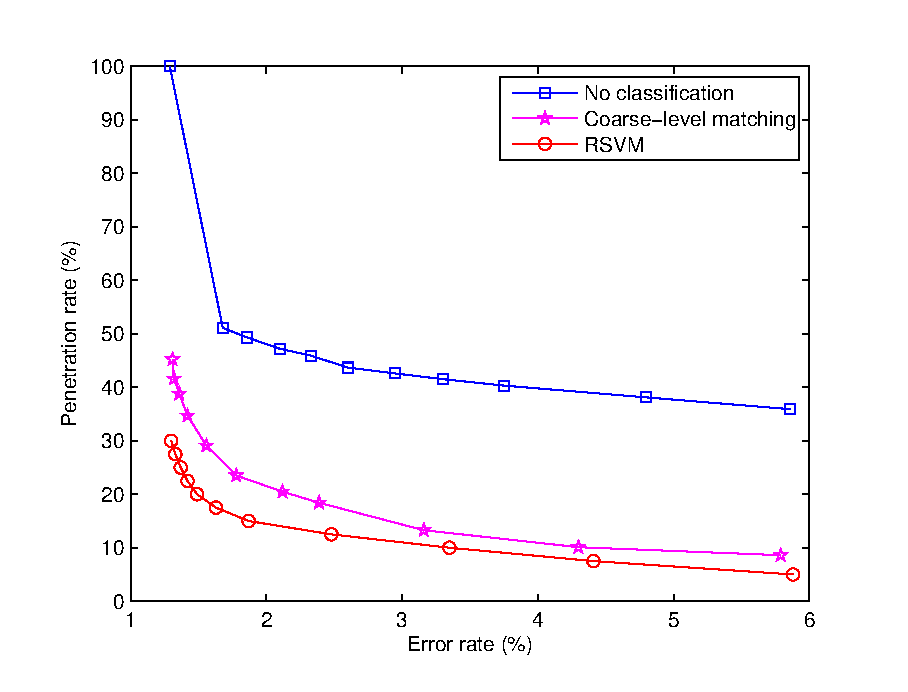
\includegraphics[width=\linewidth]{ch-experiment/figures/recognition}
\caption{Penetration rate and error rate with different matching strategies}
\label{fig:experiment:recognition}
\end{center}
\end{figure}

Figure ~\ref{fig:experiment:recognition} shows the results in a single plot.

% Table generated by Excel2LaTeX from sheet 'Sheet2'
\begin{table}[htbp]
  \centering
  \caption{Running time comparison of the three 3D palmprint recognition approaches}
    \begin{tabular}{lrrr}
    \toprule
          & No classification & Coarse-level matching & RSVM \\
    \midrule
    \multicolumn{1}{p{5cm}}{Once feature extraction time} & 112ms & 136ms & 136ms \\
    \multicolumn{1}{p{5cm}}{Once dimensionality reduction time} & 0ms   & 0.1ms & 0.1ms \\
    \multicolumn{1}{p{5cm}}{Ranking or coarse matching time for all templates in database} & 0ms   & 0.5ms & 1.56ms \\
    \multicolumn{1}{p{5cm}}{Once matching time by MCI} & 0.86ms & 0.86ms & 0.86ms \\
    \multicolumn{1}{p{5cm}}{Total running time for one probe testing} & 456ms & 292.09ms & 240.86ms \\
    \bottomrule
    \end{tabular}%
  \label{tab:experiment:time}%
\end{table}%



Table ~\ref{tab:experiment:time} shows the difference in time consumption for one probe. Due to the lower penetration rate, the running times are greatly reduced.


\chapter{Conclusions\label{ch:conclusion}}

\section{Summary}
% In this work, we explain how to use the puthesis.cls class file and the accompanying template.

In this dissertation, the authentication process are improved using 3D features. The features are stable in samples from a single person over time and distinguishable among samples from different people.

Three features adopted are Maximum Depth of palm center, Horizontal Cross-section Area and Radial Line Length from the centroid to the boundary of 3D palmprint horizontal cross-section of different levels. These cannot be extracted from 2D palmprints and are not correlated with local features, such as line and texture features. To make these global features efficient for use in coarse classification, we treat them as a multi-dimensional vector and use OLDA to map it to a lower dimensional space.

We then improve the efficiency of 3D palmprint recognition using two proposed approaches, coarse-level matching and RSVM, both of which significantly reduce the penetration rate during retrieval.

Experiments are conducted on an existing 3D palmprint database of 8,000 samples. The results show that the proposed method is able to achieve an reasonable performance.
 % Conclusion
%!TEX root = chapter-conclusion.tex
\section{Future Work}

As shown in Chapter ~\ref{ch:experiment}, the error rate in recognition using only the (Maximum Depth, Horizontal Cross-section Area, Radial Line Length are much higher than the cases when Mean Curvature Image is used. The problem with the latter one is its computation time.

The most interesting direction for future work is to find more descriptive and efficient features for the 3D ROI. % Future work


% include your .bib file
\bibliographystyle{unsrt}
\bibliography{thesis}

\appendix % all chapters following will be labeled as appendices
%!TEX root = ../thesis.tex
\chapter{Core Matlab Code\label{ch:code}}

\singlespacing

Create large arrays without asking for contiguous memory.

\begin{minted}[fontsize=\small,frame=lines,linenos]{matlab}
function result = createArrays(nArrays, arraySize, datatype)
%CREATEARRAYS
% This creates an cell array which does NOT require
% contiguous memory.
%
% To use it:
%   myArray = createArrays(numberOfArrays, [x y], 'single');
%
% To access the elements:
%   myArray{1}{2,3} = 10;
%   myArray{1} = zeros(500, 800, 'single');
    result = cell(1, nArrays);
    for i = 1 : nArrays
        result{i} = zeros(arraySize, datatype);
    end
end
\end{minted}

\clearpage

Code to find the reference plane.

\begin{minted}[fontsize=\small,frame=lines,linenos]{matlab}
function [ d_ref ] = find_ref_plane( roi )
%FIND_REF_PLANE Find the depth of reference plane of an ROI
%   Detailed explanation goes here

	[~,roi_size] = size(roi);

	refplane = roi(1:(roi_size*0.25),(roi_size*0.25):(roi_size*0.9));

	d_ref = max(max(refplane));

end
\end{minted}

\clearpage

Code to extract the X coordinates from original data.
\begin{minted}[fontsize=\small,frame=lines,linenos]{matlab}
clear;

prefix = '..\..\3D_palm';

%% File to process
load_dir = [prefix filesep '3DPalm_xyz'];
file_mask = [load_dir filesep '*.dat'];
file_list = dir(file_mask);
file_list = char({file_list.name});

%% Get X coordinates from file
tic;
dat_file = reshape(dlmread([load_dir filesep file_list(1,:)]),768,576,3);
palmX=dat_file(:,1,1);

%% Save result to file
save_dir = ['output'];
save([save_dir filesep '3Dpalm_x.mat'],'palmX');
toc;
\end{minted}

\clearpage

Code to remove outliers from a vector.

\begin{minted}[fontsize=\small,frame=lines,linenos]{matlab}
function [b,idx,outliers] = deleteoutliers(a,alpha,rep);
% [B, IDX, OUTLIERS] = DELETEOUTLIERS(A, ALPHA, REP)
% 
% For input vector A, returns a vector B with outliers (at the
% significance level alpha) removed. Also, optional output 
% argument idx returns the indices in A of outlier values. Optional
% output argument outliers returns the outlying values in A.
%
% ALPHA is the significance level for determination of outliers.
% If not provided, alpha defaults to 0.05.
% 
% REP is an optional argument that forces the replacement of
% removed elements with NaNs to presereve the length of a.
%
% This is an iterative implementation of the Grubbs Test that
% tests one value at a time. In any given iteration, the tested 
% value is either thehighest value, or the lowest, and is the
% value that is furthest from the sample mean. Infinite elements
% are discarded if rep is 0, or replaced with NaNs if rep is 1.
% 
% Appropriate application of the test requires that data can be
% reasonably approximated by a normal distribution. For reference,
% see:
% 1) "Procedures for Detecting Outlying Observations in Samples,"
%     by F.E. Grubbs; Technometrics, 11-1:1--21; Feb., 1969, and 
% 2) _Outliers in Statistical Data_, by V. Barnett and
%    T. Lewis; Wiley Series in Probability and Mathematical
%    Statistics; John Wiley & Sons; Chichester, 1994.
% A good online discussion of the test is also given in NIST's
% Engineering Statistics Handbook:
% http://www.itl.nist.gov/div898/handbook/eda/section3/eda35h.htm

if nargin == 1
	alpha = 0.05;
	rep = 0;
elseif nargin == 2
	rep = 0;
elseif nargin == 3
	if ~ismember(rep,[0 1])
		error('Please enter a 1 or a 0 for optional argument rep.')
	end
elseif nargin > 3
	error('Requires 1,2, or 3 input arguments.');
end

if isempty(alpha)
	alpha = 0.05;
end

b = a;
b(isinf(a)) = NaN;

%Delete outliers:
outlier = 1;
while outlier
	tmp = b(~isnan(b));
	meanval = mean(tmp);
	maxval = tmp(find(abs(tmp-mean(tmp))==max(abs(tmp-mean(tmp)))));
	maxval = maxval(1);
	sdval = std(tmp);
	tn = abs((maxval-meanval)/sdval);
	critval = zcritical(alpha,length(tmp));
	outlier = tn > critval;
	if outlier
		tmp = find(a == maxval);
		b(tmp) = NaN;
	end
end
if nargout >= 2
	idx = find(isnan(b));
end
if nargout > 2
	outliers = a(idx);
end
if ~rep
	b=b(~isnan(b));
end
return

function zcrit = zcritical(alpha,n)
%ZCRIT = ZCRITICAL(ALPHA,N)
% Computes the critical z value for rejecting outliers (GRUBBS TEST)
tcrit = tinv(alpha/(2*n),n-2);
zcrit = (n-1)/sqrt(n)*(sqrt(tcrit^2/(n-2+tcrit^2)));
\end{minted}
\clearpage

Code for batch feature extraction.

\begin{minted}[fontsize=\small,frame=lines,linenos]{matlab}
clear;

%% Files to process
save_dir = ['output'];

use_original_data = true;
% Toggle this for data source selection
% use_original_data = false;

if (use_original_data)
    data_dir = ['..' filesep 'rawdata'];
    file_mask = [data_dir filesep '*.zonly'];
    sample_width = 768;
    sample_height = 576;
    roi_size = 400;
else
    data_dir = ['..' filesep 'rawdata' filesep 'roi'];
    file_mask = [data_dir filesep '*.dat'];
    sample_width = 128;
    sample_height = 128;
    roi_size = 128;
end

file_list = dir(file_mask);
file_list = char({file_list.name});

num_of_samples = length(file_list);
sample_per_person = 10;
num_of_people = num_of_samples/sample_per_person;
% Toggle this for limited number of files
// num_of_people = 100;

feature_dimension = roi_size;
% feature_dimension = roi_size*roi_size;

features = zeros(num_of_people*sample_per_person,feature_dimension);

%% Parallel read files
tic;
for current_person = 1:num_of_people
    disp(['Loading data from ' num2str(current_person) ' of \
		' num2str(num_of_people) ' people.']);
    for current_sample = 1:sample_per_person
        file_id = (current_person - 1) * 10 + current_sample;
        sample_filename = strtrim([data_dir filesep file_list(file_id,:)]);
        
        mat = file2matrix(sample_filename, sample_width, sample_height);
        
        if (use_original_data)
            % Crop ROI from original data
            mat = mat(235:(234+roi_size),69:(68+roi_size));
        end;
        
        % Extract feature for this sample
        features(file_id,:) = calc_feature(mat);
    end
end

save(['output' filesep 'features.mat'], 'features');
toc;
\end{minted}
\clearpage

Code for curvature extraction.

\begin{minted}[fontsize=\small,frame=lines,linenos]{matlab}
function [K,H,Pmax,Pmin] = surfature(X,Y,Z),
% SURFATURE -  COMPUTE GAUSSIAN AND MEAN CURVATURES OF A SURFACE
%   [K,H] = SURFATURE(X,Y,Z), WHERE X,Y,Z ARE 2D ARRAYS OF POINTS
%   ON THE SURFACE.  K AND H ARE THE GAUSSIAN AND MEAN CURVATURES,
%   RESPECTIVELY.
%
%   SURFATURE RETURNS 2 ADDITIONAL ARGUEMENTS,
%
%   [K,H,Pmax,Pmin] = SURFATURE(...), WHERE Pmax AND Pmin ARE THE
%   MINIMUM AND MAXIMUM CURVATURES AT EACH POINT, RESPECTIVELY.


% First Derivatives
[Xu,Xv] = gradient(X);
[Yu,Yv] = gradient(Y);
[Zu,Zv] = gradient(Z);

% Second Derivatives
[Xuu,Xuv] = gradient(Xu);
[Yuu,Yuv] = gradient(Yu);
[Zuu,Zuv] = gradient(Zu);

[Xuv,Xvv] = gradient(Xv);
[Yuv,Yvv] = gradient(Yv);
[Zuv,Zvv] = gradient(Zv);

% Reshape 2D Arrays into Vectors
Xu = Xu(:);   Yu = Yu(:);   Zu = Zu(:); 
Xv = Xv(:);   Yv = Yv(:);   Zv = Zv(:); 
Xuu = Xuu(:); Yuu = Yuu(:); Zuu = Zuu(:); 
Xuv = Xuv(:); Yuv = Yuv(:); Zuv = Zuv(:); 
Xvv = Xvv(:); Yvv = Yvv(:); Zvv = Zvv(:); 

Xu          =   [Xu Yu Zu];
Xv          =   [Xv Yv Zv];
Xuu         =   [Xuu Yuu Zuu];
Xuv         =   [Xuv Yuv Zuv];
Xvv         =   [Xvv Yvv Zvv];

% First fundamental Coeffecients of the surface (E,F,G)
E           =   dot(Xu,Xu,2);
F           =   dot(Xu,Xv,2);
G           =   dot(Xv,Xv,2);

m           =   cross(Xu,Xv,2);
p           =   sqrt(dot(m,m,2));
n           =   m./[p p p]; 

% Second fundamental Coeffecients of the surface (L,M,N)
L           =   dot(Xuu,n,2);
M           =   dot(Xuv,n,2);
N           =   dot(Xvv,n,2);

[s,t] = size(Z);

% Gaussian Curvature
K = (L.*N - M.^2)./(E.*G - F.^2);
K = reshape(K,s,t);

% Mean Curvature
H = (E.*N + G.*L - 2.*F.*M)./(2*(E.*G - F.^2));
H = reshape(H,s,t);

% Principal Curvatures
Pmax = H + sqrt(H.^2 - K);
Pmin = H - sqrt(H.^2 - K);
\end{minted}
\clearpage

Code to test feature performance.

\begin{minted}[fontsize=\small,frame=lines,linenos]{matlab}
%% Load features
load(['output' filesep 'features.mat']);

[total,~] = size(features);

%% Split into training set and testing set
training_id=unique([
    1:10:total
    2:10:total
    3:10:total
    4:10:total
    5:10:total
    6:10:total
    ]);

trainingset = features(training_id,:);

test_id=unique([
    7:10:total
    8:10:total
    9:10:total
    10:10:total
    ]);

testingset = features(test_id,:);

%% Find match for each test input
nearest_id = knnsearch(trainingset, testingset, 'k', 10);

%% Interpret the match to person
[total_training,~] = size(trainingset);
training_sample_per_person = total_training / total * 10;
nearest_person = ceil(nearest_id/training_sample_per_person);

%% Check performance
[total_testing,~] = size(testingset);
testing_sample_per_person = total_testing / total * 10;
for i = 1:total_testing
    correct(i) = eq(nearest_person(i),ceil(i/testing_sample_per_person));
end
correct = correct';

accuracy = sum(correct)/total_testing
\end{minted}
\clearpage

Code to extract shape features.

\begin{minted}[fontsize=\small,frame=lines,linenos]{matlab}
function extractShapeF()

sizeH = 200; %
sizeW = 200; %
lnum = 8;

pixDis = 0.28;
% load facesMatrix64.mat;
temp = pixDis * ((sizeH-2)/2+0.5);
[X,Y] = meshgrid(-temp : pixDis : temp);

fid = fopen('../rawdata/Sub3D_I_3_0.dat', 'r');
% fid = fopen('../rawdata/Sub3D_II_100_0.dat', 'r');
Z = fread(fid, [sizeH,sizeW], 'double');
fclose(fid);
[fx, fy] = gradient(Z);
fxy = fx.^2 + fy.^2;
noiseP = find(fxy>0.1); % 0.1 used for corrected and smoothed Sub3D, 1 used for original Sub3D
flag = ones(sizeH, sizeW); %1 for valid point, 0 for invalid point
flag(noiseP) = 0;
flag = 1 - flag;
se = strel('disk',5);  
flag = imdilate(flag, se);
flag = 1 - flag;
noiseP = find(flag==0);
meanZ = sum(sum(Z .* flag)) / (sizeH*sizeW - length(noiseP));
Z(noiseP) = 5;
%neend't smooth
% Z = smooth(Z, 7);

%%for show the mask which get rid of bad quality region
% flag(1,:) = 0; flag(end,:) = 0;
% flag(:,1) = 0; flag(:,end) = 0;
% imshow(flag');

%calculate the reference 0 plane
% use Z(6:35, 65:136) for calculate the mean value as reference 0
refRect = Z(6:35, 65:136);
refFlag = flag(6:35, 65:136);
refVal = sum(sum(refRect .* refFlag)) / sum(sum(refFlag));
Z = Z - refVal;

%search the min point in Z(65:190, 41:160)
rectforMin = Z(65:190, 41:160);
rectforMin(1:35, 1:25) = 5;
rectforMin(1:35, end-25:end) = 5;
% flagforMin = Z(65:190, 41:160);
palmH = min(min(rectforMin));
ind = find(Z == palmH);
% Z(ind) = 5;

% %find the level regions from 0 to deepest point 
% %find the region > 0
% palmH = -palmH;
% Z = -Z;
% Ln = 8;
% step = palmH / Ln;
% levelH = [0:step:palmH];
% for i = 1:Ln
%     L0 = zeros(sizeH, sizeW);
%     L0( find( Z>=levelH(Ln-i+1) ) ) = 1;
%     %the 1st level
%     if i==1
%         [L,num] = bwlabel(L0);
%         if num > 1
%             for j = 1:num
%                 indL = find(L==j);
%                 if length(find(indL==ind)) > 0
%                     L0(:,:) = 0;
%                     L0(indL) = 1;
%                 end
%             end
%         end
%         Lp = L0;
%         L0 = logical(L0');  
%         [x, y] = find(L0);
%         temp = find(L0);
%         mx = mean(x);
%         my = mean(y);
% 
% %         saveIm(L0, i);
%         figure;
%         imshow(L0);
%     else
%         %dilate the Lp (previous level) and than & with L0
%         se = strel('disk',35 - 3*i);  
%         L1 = imdilate(Lp, se);
%         L0 = L0 & L1;
%         Lp = L0;
%         L0 = L0';   
% %         saveIm(L0, i);
%         figure;
%         imshow(L0);
%     end    
% end

%for show
im_level = zeros(sizeH, sizeW); %for show the levels
%find the level regions from 0 to deepest point 
%find the region > 0
palmH = -palmH;
Z = -Z';
Ln = 8;
step = palmH / Ln;
levelH = [0:step:palmH];
for i = 1:Ln
    L0 = zeros(sizeH, sizeW);
    L0( find( Z>=levelH(Ln-i+1) ) ) = 1;
    %the 1st level
    if i==1
        [L,num] = bwlabel(L0);
        if num > 1
            for j = 1:num
                indL = find(L==j);
                if length(find(indL==ind)) > 0
                    L0(:,:) = 0;
                    L0(indL) = 1;
                end
            end
        end
        Lp = L0;
        [x, y] = find(L0);
        temp = find(L0);
        mx = round(mean(x));
        my = round(mean(y));
        im_level(temp) = 155;

%         saveIm(L0, i);
%         figure;
%         imshow(L0);
    else
        %dilate the Lp (previous level) and than & with L0
        se = strel('disk',35 - 3*i);  
        L1 = imdilate(Lp, se);
%         figure; imshow(Lp);
%         figure; imshow(L1);
        L0 = L0 & L1;
%         figure; imshow(L0);
        Ltemp = L0 - Lp;
%         figure; imshow(Ltemp);
        Lp = L0; 
        temp = find(Ltemp);
        im_level(temp) = 255-(i-1)*30;
%         saveIm(L0, i);
%         figure;
%         imshow(L0);
    end    
end

im_level = uint8(im_level);
% imshow(im_level);
% imwrite(im_level, 'figures/im_levels.bmp');

line_401 = imread('figures/line_all.bmp');
line_200 = line_401(201-mx+1:201-mx+1+199, 201-my+1:201-my+1+199);
% imshow(line_200);
temp = find(line_200);
im_level(temp) = 20;
im_level(mx, my) = 255;
figure;
imshow(im_level);
imwrite(im_level, 'figures/im_levels_line_4.bmp');
a = 0;

% %%% Z(6:35, 65:136) = 0;
% Z(6:35, 65) = 1;
% Z(6:35, 136) = 1;
% Z(6, 65:136) = 1;
% Z(35, 65:136) = 1;

% figure;
% mesh(X,Y,Z);
% daspect([1 1 1]);
% view([90 90]);

a = 0;

%-----------------------------------------------------------------
function saveIm(data, nlevel)
filename = ['../rawdata/bmp/Sub3D_I_4_9', '_' num2str(nlevel), '.bmp'];
imwrite(data, filename);


function [z] = smooth(z, fs)
% z -- 128*128
% n -- filter size
t = floor(fs/2)-1;
for i = 0:t;
    [m,n] = size(z);
    z = [z(:, 2*i+1) z(:,:) z(:, n-2*i)];
end

for i = 0:t;
    [m,n] = size(z);
    z = [z(2*i+1, :); z(:,:); z(m-2*i, :)];
end

h = ones(fs,fs)/(fs*fs);
z = filter2(h, z, 'valid');
\end{minted}
\clearpage
% %!TEX root = ../thesis.tex
\chapter{Printing and Binding\label{ch:printing}}

\section{Printing}

For the library copies of your dissertation, you must use archival quality printing and binding. This means acid-free paper, containing at least 25\% cotton fiber. Triangle Repocenter on Nassau Street in Princeton offers both 25\% cotton paper and 100\% cotton paper. Most people choose the 25\% cotton paper, and this is generally recommended by the binders. The 100\% copy paper is somewhat thicker and the extra expense is unnecessary. 

Triangle offers online submission of your printing and binding order at: \url{http://triangleprinceton.com/collegiatebinding/thesis/}. If you request binding from them, they will deliver the paper copies to Smith-Shattuck Bookbinding for you and allow you to pick up the completed copies at their store on Nassau Street. The whole process takes 2-3 business days, but check with them in advance during the busy thesis-printing season in April and May. 

Currently, your printed and bound dissertation copies can be single spaced. Only the electronic copy submitted to ProQuest must be double spaced. All copies must be printed single-sided, with specific margins. 

\section{Binding}

An archival-quality sewn binding is required for the library copies of your dissertation. Smith-Shattuck Bookbinding is highly recommended, and is used by most students. Triangle Repocenter will send your copies there for you, greatly simplifying the process, but you can call Smith-Shattuck with special requests. 

The ``library standard'' sewn binding is sufficient for the copies to be sent to Mudd Library. It uses a black buckram cloth cover, which is the most popular option. For extra copies for yourself and your family members, you can choose ``buckram roundback binding'', which adds decorative lines on the spine, and printing of the title and author on the front cover. For a small additional fee, you can include the Princeton University shield on the front cover and a ribbon bookmark. Leather covers are also available. See Smith-Shattuck's website for more details at: \url{http://www.thesisbookbinding.com/}. 

\end{document}

